In 1895, Oscar Wilde wrote The Importance of Being Earnest, ridiculing Victorian conventions. Far from these considerations, it was shown that the biological relevance of being earnestness is very dependent on the sex of an organism and the natural mating system of the species to which it belongs \citep{Wade80,Darwin08,Shuster09,Tilquin16}. The same holds when one substitutes this first name for its French counterpart "Constant". Since Biology is about being adapted, its fitness may rely on constantly changing its phenotype when the environment varies, or, on the contrary, may require one to target one or few (in the case of balancing selection) constant optimal phenotypic values or ratios. For illustrative purpose, let us slip ourself in the shoes of Alice pilgriming in her Wonderland. When she suddenly grows up, her whole body extends, not only one specific part \citep{Carroll66}. Were it not to be the case, this body would appear completely unfit due to simple physical properties such as the Fundamental principle of the dynamics of rotation regarding joints. Such conservation of scaling and relative proportions has been extensively studied for one century since the seminal work of D'arcy Thompson \citep{Darcy92} through the concept of allometry \citep{Gould66,Cheverud82,Damuth01,Dill11}, shedding light on these scaling laws \citep{West05}, their range of variation and the reasons behind both their variability and similarity \citep{Pelabon14}. We have shown previously that such constancy ratios should also been maintained along metabolic pathways since the final flux depends on the efficiency of all proteins involved in it. Consequently, it seems relevant to evaluate how this need for regularity impacts population genetics. This is what we propose to address in the following pages.

\subsection{{An introduction on epistasis, complexity and the need for complementarity}\label{sec:Intro-Epi-Complex}}

\subsubsection{About complex genetic interactions}

‘‘\textit{On rencontre sa destinée souvent par les chemins qu'on prend pour l'éviter}''.

Jean de la Fontaine

\begin{figure}[h!]
    \centering
    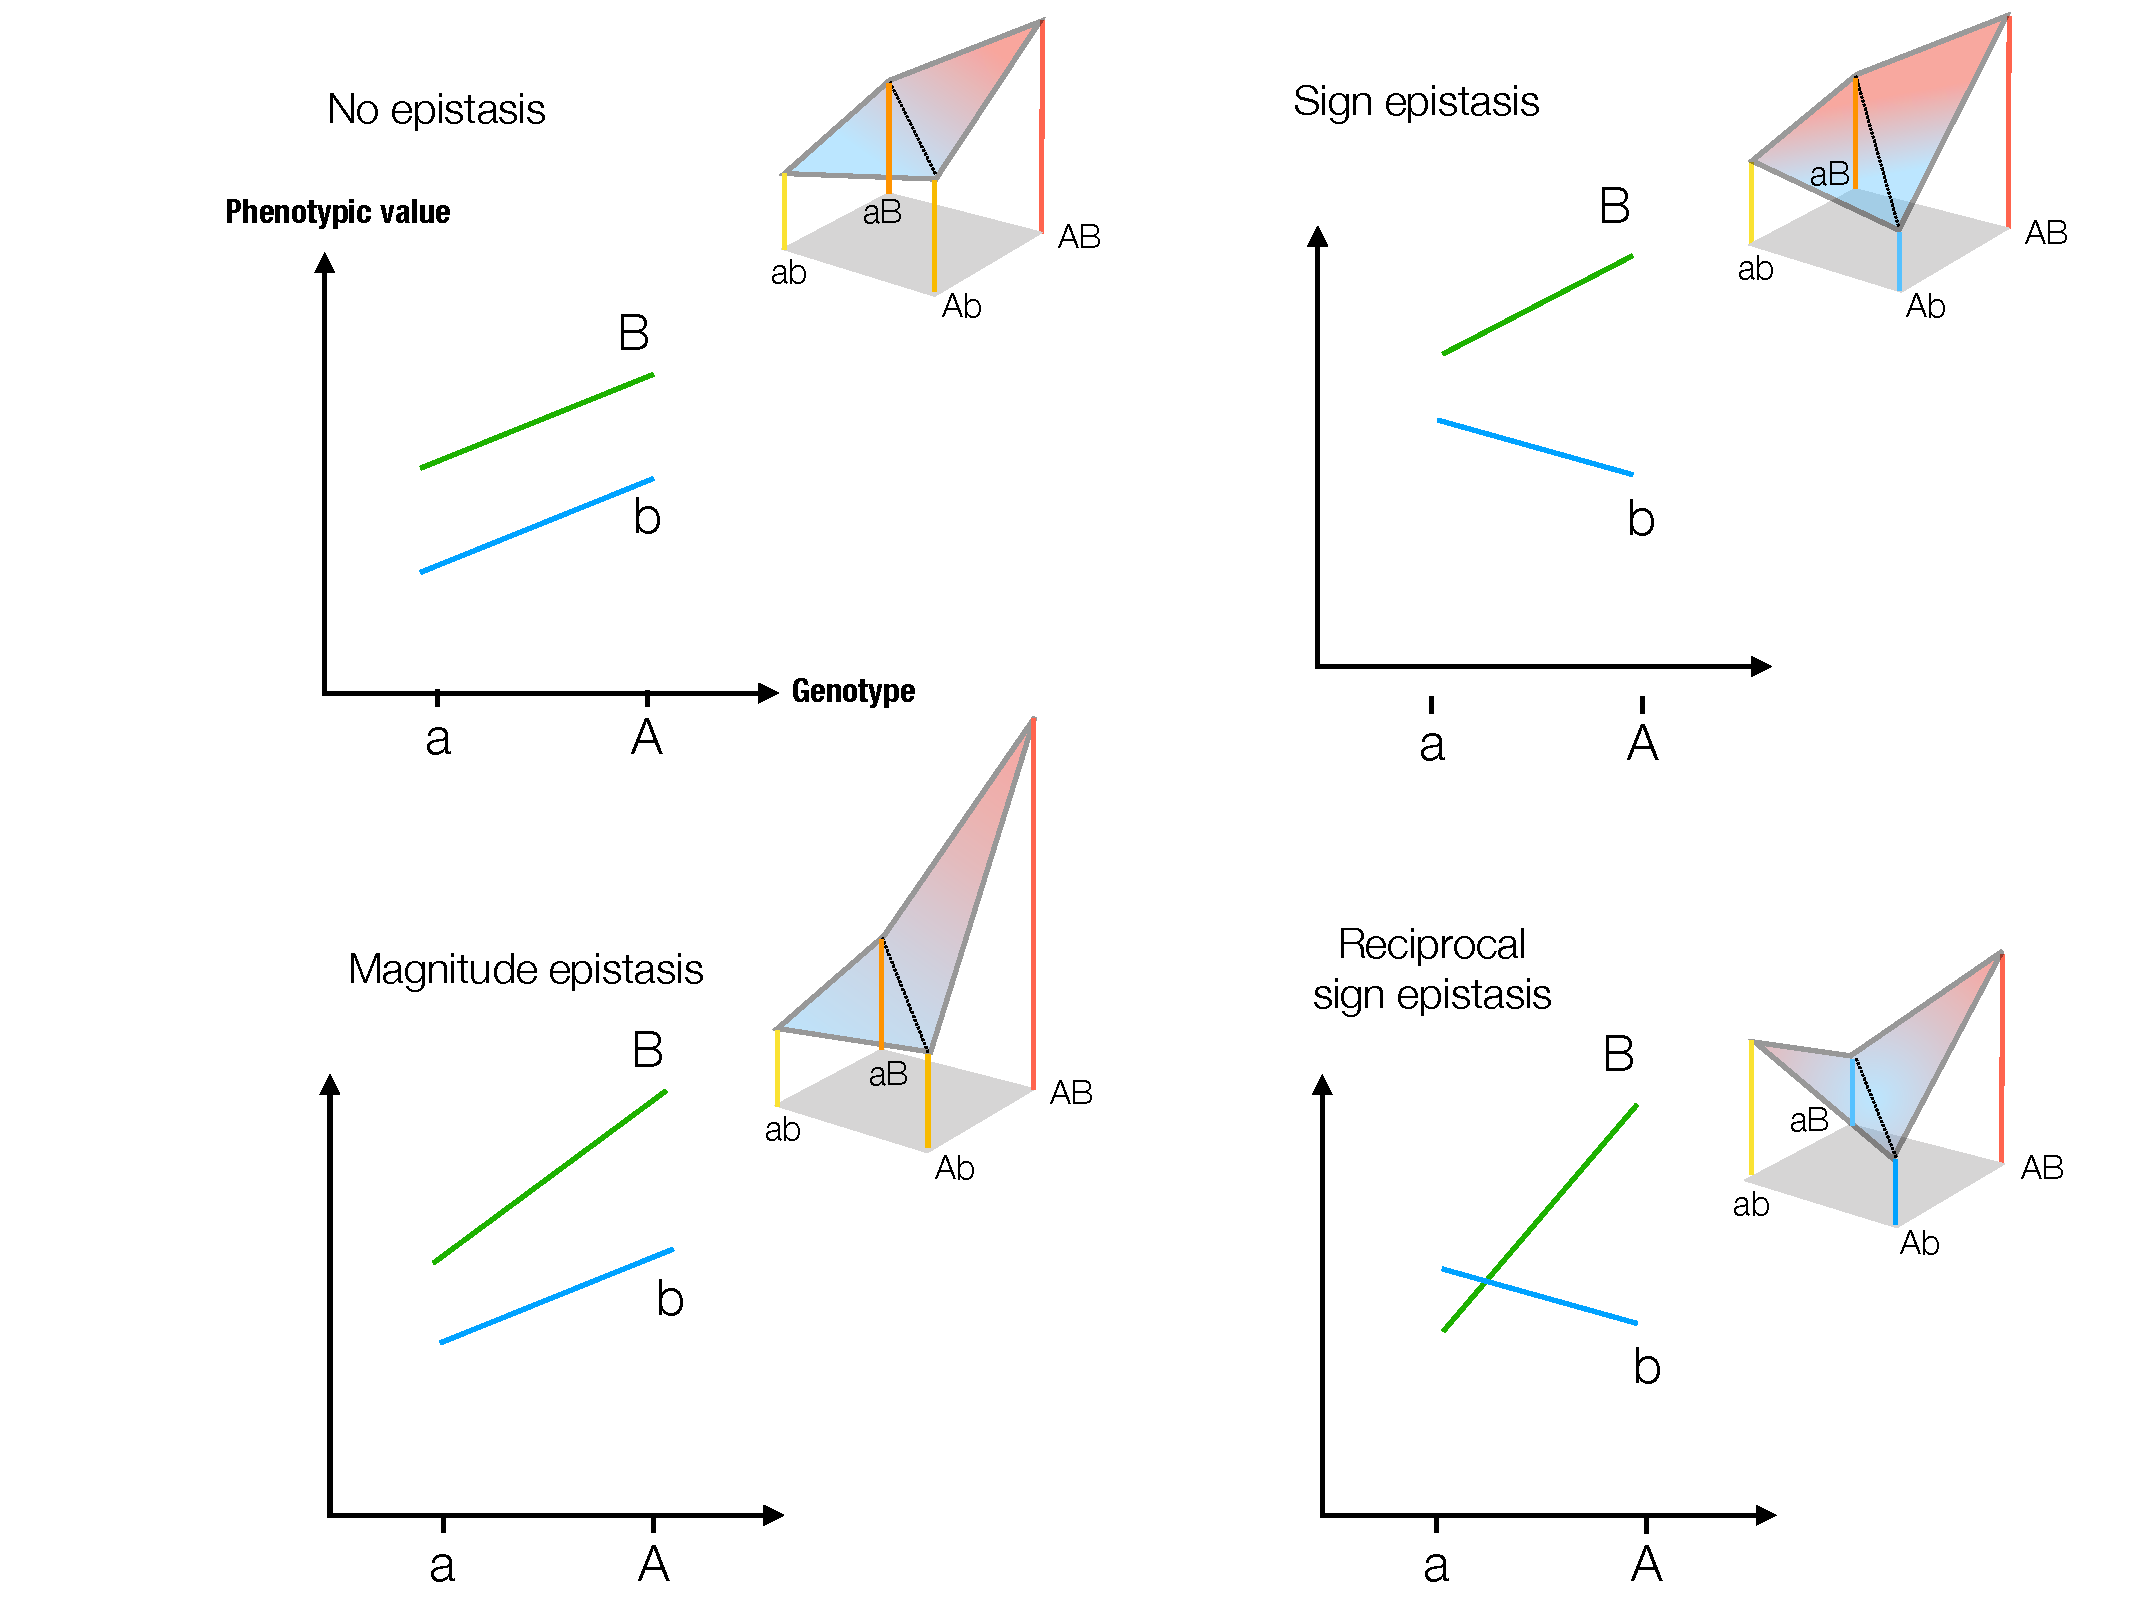
\includegraphics[scale=0.45,trim=3cm 0cm 0cm 0cm,clip]{pics/Epistasis/2D-epistasis.pdf}
    \caption{Main types of two-locus epistasis. First, no epistasis corresponds to the simple additivity model where loci (a/A or b/B) contribute the same amount to the trait no matter the value of a second locus involved in the trait. Magnitude epistasis depicts the case where synergistic or antagonistic effects come into play so that the effect of the combination is respectively increased or decreased compared to the expected additivity. With sign epistasis, the sign of the contribution brought by the second locus changes with the value of the first locus, which narrows the path towards the highest fitness. Reciprocal sign epistasis coincides with an extreme case of sign epistasis where both intermediate mutants (aB or Ab) are deleterious, giving birth to a fitness valley separating two local peaks.}
    \label{fig:2D-epistasis}
    \vspace{-0.5cm}
\end{figure}

Epistasis (see Figure \ref{fig:2D-epistasis}) is a ubiquitous phenomenon in which the effect of a mutation differs depending on the genetic background in which it occurs \citep{Bateson09,Phillips08,Domingo19}. As \citet{Weinreich13} pointed out, it is a measure of our ‘‘surprise" insofar as we \textit{a priori} expect mutational effects to be additive \citep{Phillips08,Domingo19}. Epistasis has long been known to occur between pairwise mutations where the combined effect between them results in a phenotype or a fitness not being the sum of that they would have in isolation from one another \citep{Bateson09}. If Adaptation can sometimes still occur through few genetic changes \citep{Orr05}, such epistatic interactions in general comes with several consequences. Forasmuch as it influences genetic architecture \citep{Hermisson03,Domingo19,Sella19}, it often narrows the path towards adaptive phenotypes \citep{Poelwijk07} and may even create fitness valleys under certain circumstances called reciprocal sign epistasis \citep{Weinreich05b,Poelwijk11} - see Figure \ref{fig:2D-epistasis} for visual explanations.

Because of the process of genetic drift \citep{Wright30,Kimura58,Ohta92,Sella09} that entails a mutational load \citep{Haldane37,Muller50,Agrawal12}, lower effective population sizes (as was shown again for enzyme efficiencies in our work - see \ref{sec:Results}) are, on average, further from the optimum phenotype. This is notably the case when a species experiences a bottleneck \citep{Wright31,Nei75} during which part of the genetic variability is lost even if adaptive. It was thus supposed that small effective population sizes could help escape from a local fitness peak by facilitating fixation of intermediate deleterious mutations \citep{Wright30,Wright32} ; therefore, subdivision in small populations should be better at finding the highest peak though they are less efficient to climb up towards this peak. In a sense, as Jean de La Fontaine once put it, one may often meet his (Adaptive) Destiny on the (Neutral) route he took to escape from It. However, introducing polymorphism and recombination disproved this conclusion \citep{Weinreich05} since combined mutations can either be found through stochastic tunneling \citep{Iwasa04b} -- whereby a population jump to the fixation of an adaptive double mutation thanks to the transient segregation of a first deleterious mutation -- or be brought together after having emerged in different lineages, and it was later shown that considering the width -- \textit{i.e.} the number of loci making up the valley -- of valleys would even reverse Wright's initial intuition with higher populations more prone to cross large fitness valleys, especially if these valleys are much alike plateaus \citep{Weissman09}.

Known as high(er)-order epistasis\footnote{see Illustrated Glossary of complex genetic interactions in Box \ref{Box-Glossary-CompInt}}, this phenomenon involving many interacting loci usually gives rise to rugged fitness landscapes \citep{Kauffman87,Kauffman89,Weinreich13} where peaks and valleys quickly follow each other in both the phenotype and the genotype spaces, as can be observed in Figure \ref{fig:NKModel}-C. Based on the NK-model (see Box \ref{Box-NKModel} to get to the nitty gritty of the model), \citet{Kauffman87} showed that such high order epistasis -- assimilated to a kind of complexity -- comes at a great cost for fitness since more ruggedness in turn increases the probability of being trapped at a local optimum \citep{Kauffman87,Geard02}, a finding that was further confirmed when accounting for the possibility of neutral mutations, through NKq and NKp models \citep{Barnett98,Newman98,Geard02}. Under certain assumptions, this model makes possible to estimate analytically the average expected mutation-selection-drift balance \citep{Weinberger91} and its mutational load counterpart, which can thus be contrasted to other such predictive frameworks.

\begin{mybox}{\begin{Note-box}
%\vspace{0.3cm}
\label{Box-Glossary-CompInt}A definition of high order epistasis\end{Note-box}}
\onehalfspacing
\textbf{High order epistasis} is the general case of epistasis where the interaction involves a great number of interacting parts owing to processes detailed in Box \ref{Box-Glossary-CompInt}. It features the effect of the genomic background on lower order interactions (see Figure \ref{fig:GlossCompInt}); noticeably, it was shown that the magnitude of epistasis sometimes seems to decline with its order \citep{Ferretti16,Weinreich18}, which means that high order interactions may be overlooked in certain cases. 
\begin{center}
    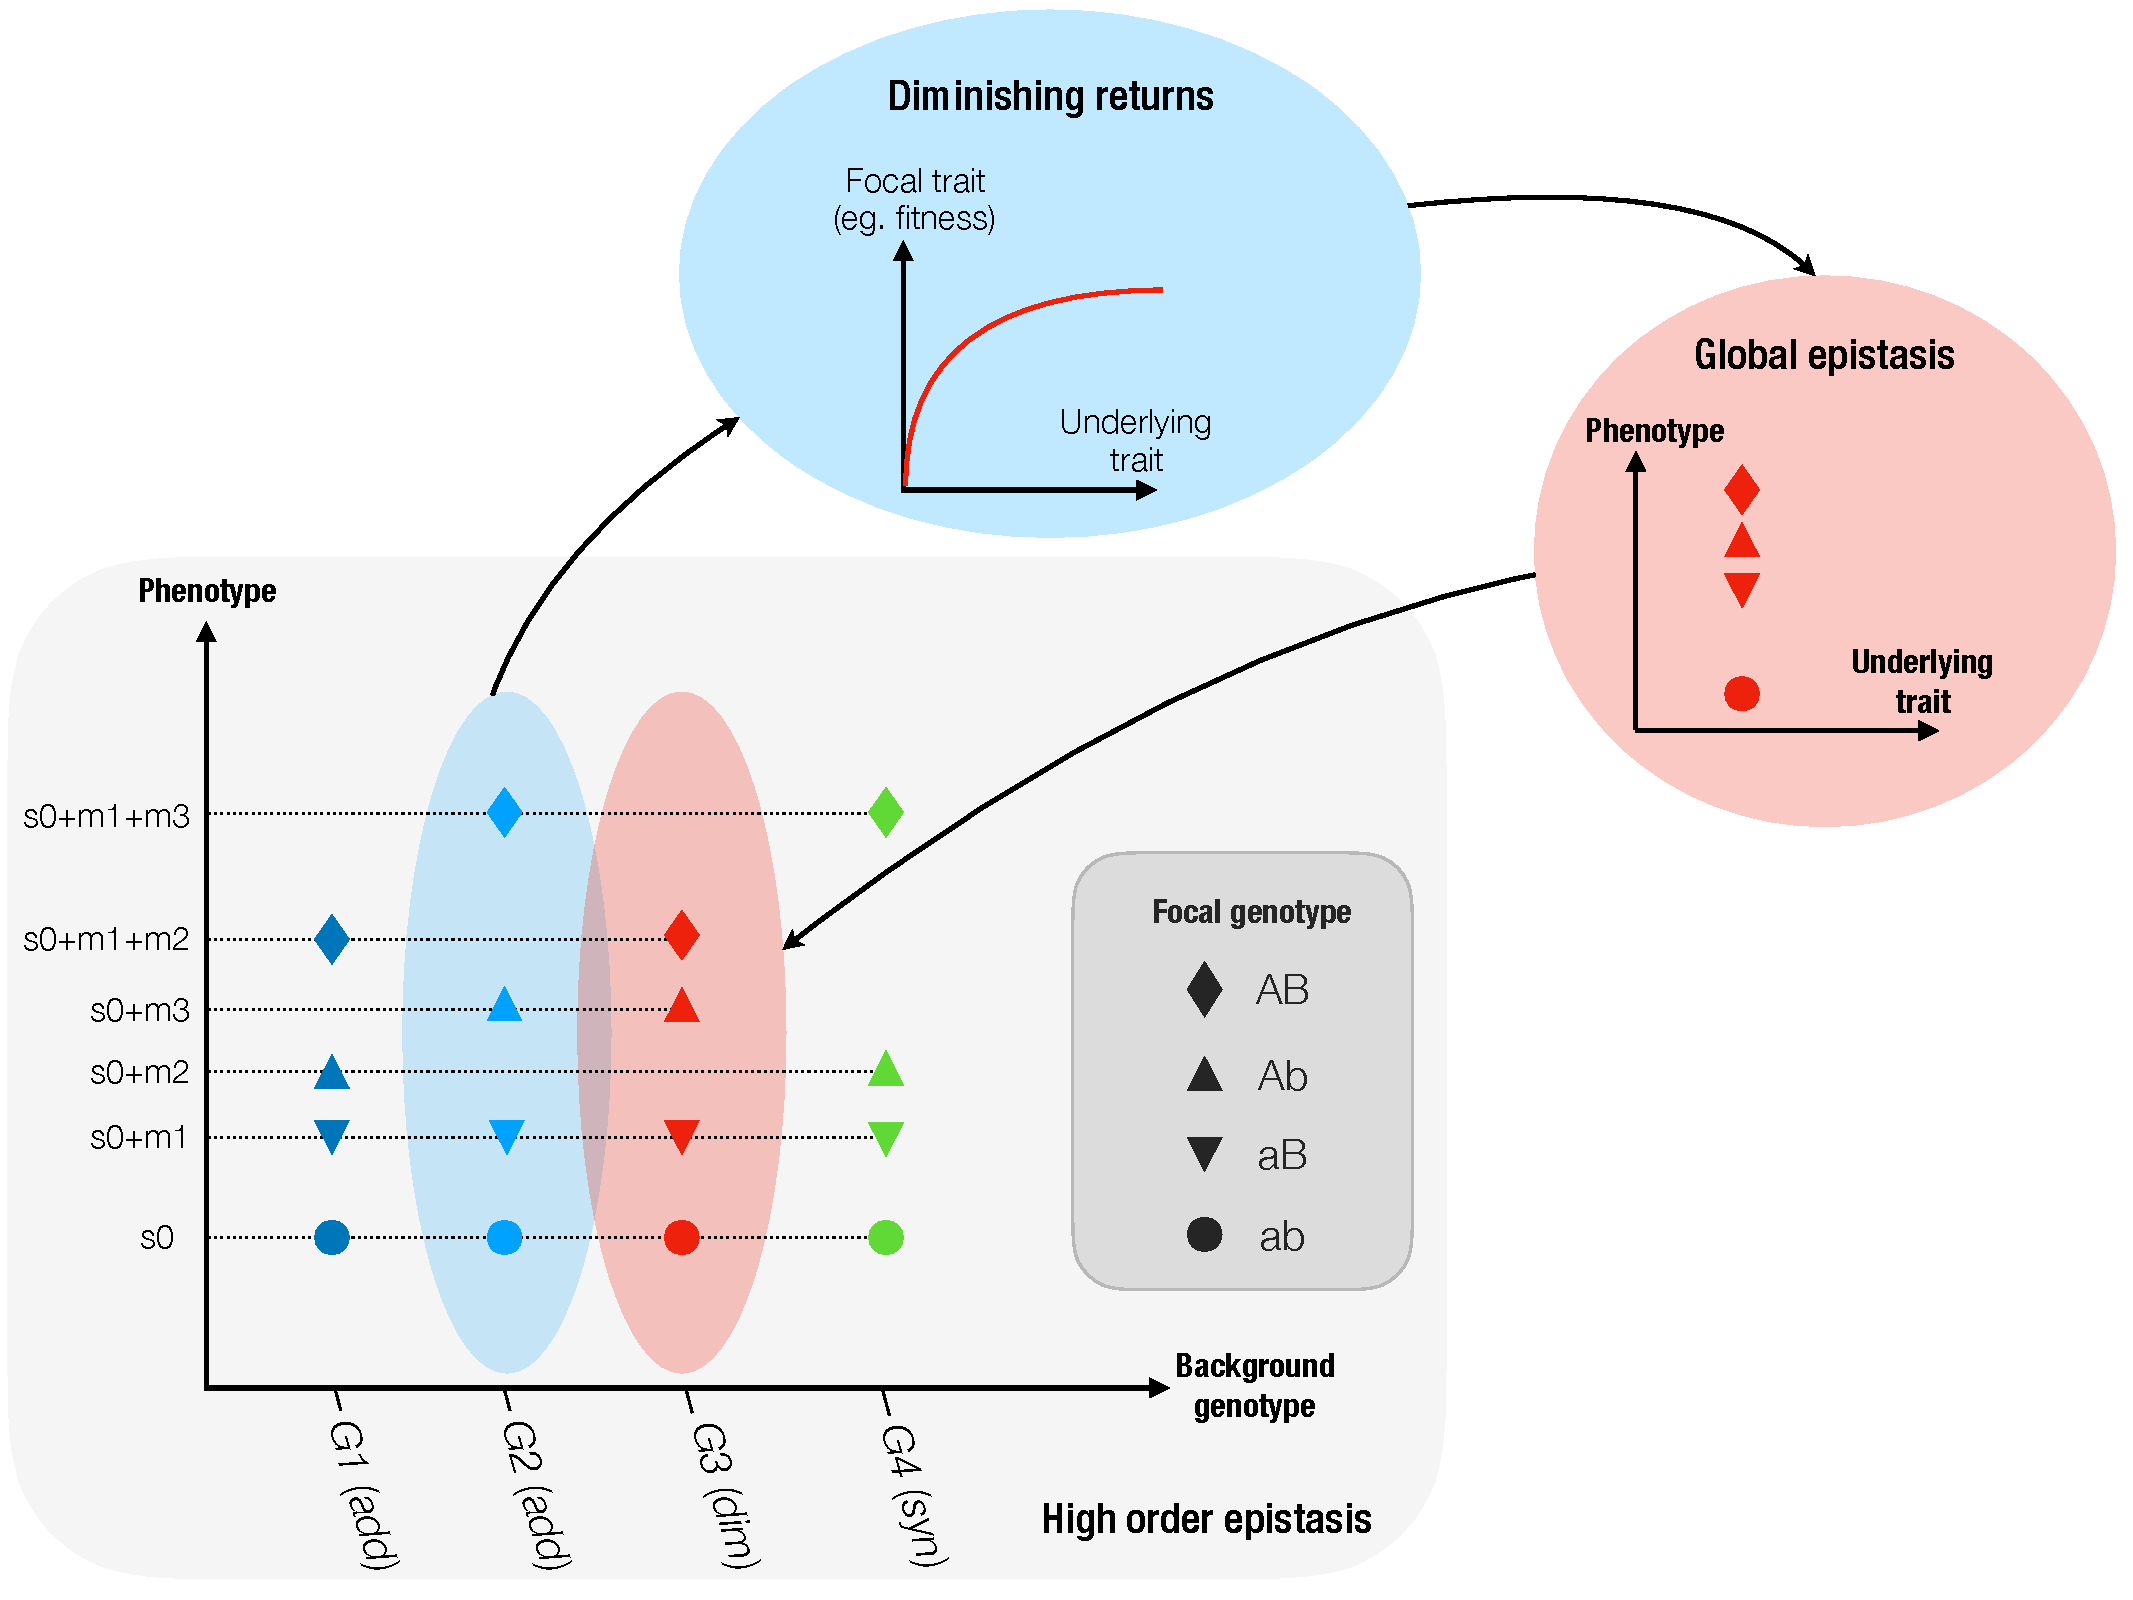
\includegraphics[scale=0.39,trim=0cm 0cm 0cm 0cm,clip]{pics/Epistasis/High-order-epistasis-sch.pdf}
    \captionof{figure}{In \textbf{High order epistasis}, the genetic background (denoted G) modifies how loci combine to produce a phenotype (\textit{eg.} $G1$ \textit{vs} $G2$, with a lower level interaction involving two loci in the picture). Synergistic epistasis ('syn', occuring in $G4$) means that mutations produce a higher effect on the phenotype than the expected additive one. Diminishing-returns epistasis ('dim') stands for any mutational interaction in which the effect of combined advantageous mutations is less than the sum of their isolated effect. As a corollary, \textbf{global epistasis} is a special case of diminishing returns epistasis ('dim', occuring in $G3$) and occurs when several loci combine additively ('add') on an underlying - possibly unobserved - trait that influences an observed trait or phenotype (including fitness) through a diminishing returns relationship.}
    \label{fig:GlossCompInt}
\end{center}
\end{mybox}

%\vspace{-0.3cm}

\begin{mybox}{\begin{Note-box}
\label{Box-Glossary-CompInt}Illustrated glossary on the processes behind high order epistasis\end{Note-box}}
\onehalfspacing
%\begin{minipage}{0.95\textwidth}
\begin{center}
    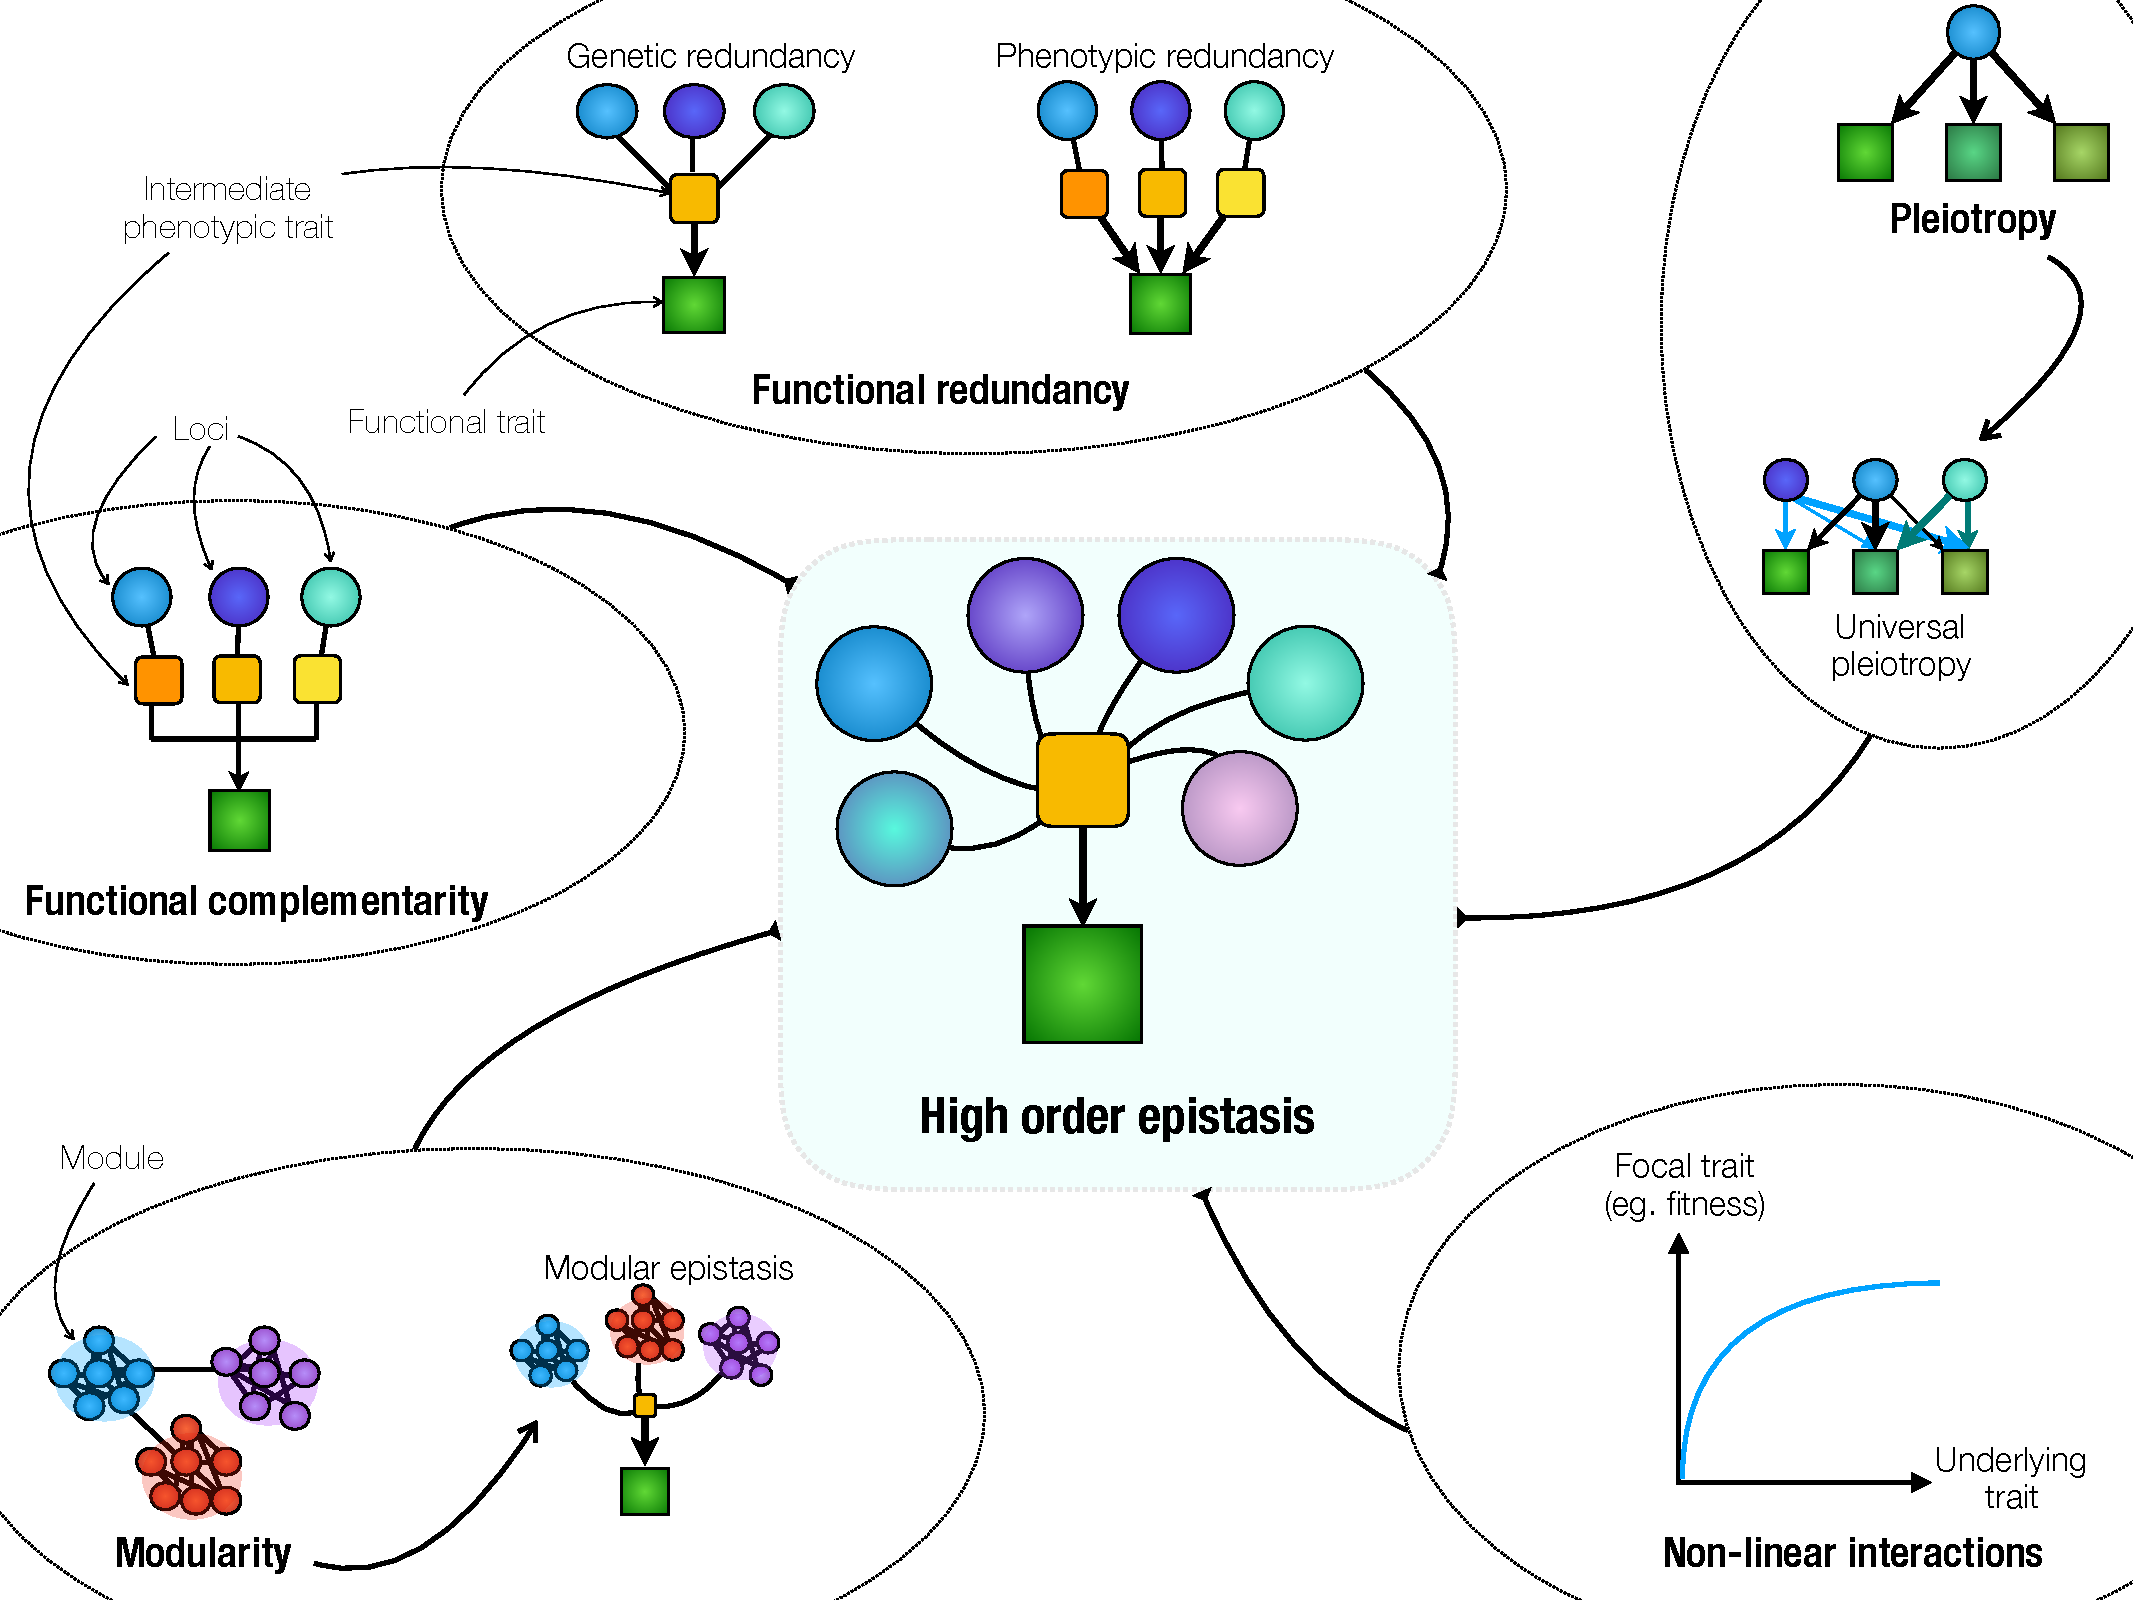
\includegraphics[scale=0.4,trim=0cm 0cm 0cm 0cm,clip]{pics/Epistasis/Genetic-interactions.pdf}
    \captionof{figure}{Summary of the genetic interactions involved in the emergence of high order epistasis. \textbf{Functional complementarity} results from the contribution of different intermediate phenotypic traits that each need be present in order to produce a functional phenotype: when different loci are involved in the intermediate traits, this gives rise to complementary epistasis (see also Figure \ref{fig:ComplementaryEpi}). This is true for example when a specific color results from the involvement of several pigments. \textbf{Functional redundancy} describes the existence of multiple ways - often involving sub-phenotypic traits (\textbf{\textit{Phenotypic redundancy}}) - to optimize a phenotypic trait (eg. concentration, affinity and catalytic rates for enzyme efficiency). \textbf{\textit{Genetic redundancy}} is also possible, with distinct loci involved in the same phenotypic trait (\textit{eg.} loci contributing to protein stability, or different genes involved in the same function) and may follow from duplication and sub-functionalization, for instance. \textbf{Pleiotropy} represents a process in which a specific locus (\textit{eg.} single residue) influences several traits at once. Owing to the numerous interactions occuring in gene newtorks, many loci are assumed to influence many traits at once: this idea has been coined \textbf{\textit{Universal pleiotropy}}. Loci - or underlying phenotypic traits - may combine through \textbf{Non-linear interactions}, akin the diminshing returns law shown here, to produce a focal trait. \textbf{Modularity} defines the existence of relatively independent modules (\textit{eg.} the arm and the leg) - in that they contribute independently to the phenotype - that are comprised of tightly interacting parts. Combined with epistasis, it extends the latter concept into \textbf{\textit{Modular epistasis}} where each functional units (modules) display purely buffering or aggravating interactions.}
    \label{fig:GlossCompInt}
\end{center}
\end{mybox}

    %\item[] Higher-order epistasis is a phenomenon where epistasis involves many different genes/residues and is used, for instance, to describe the influence of genetic background on epistasis involving two or few specific mutations.


Indeed, the influence of complexity on evolutionary trajectories and outcomes has in parallel thoroughly been addressed through the lens of Fisher's geometrical model \citep{Fisher30,Orr98,Orr00,Poon00,Martin06,Tenaillon07,Sella09,Tenaillon14}. Within this framework, epistasis builds up from the mathematical underpinnings \citep{Hartl96,Orr00,Tenaillon14,Hwang17} and the assumption of both non-linearities in the fitness landscapes\citep{Hwang17} and pleiotropy preexistence \citep{Tenaillon14} - see Box \ref{Box-FisherModel} for a description of Fisher's geometrical model and \citep{Stearns10} for a review on pleiotropy.Besides enabling to study the distribution of fitness effects \citep{Martin06,Lourenco11}, it is in principle possible through this framework to approach how complexity emerges and evolves \citep{Orr98,Martin07,Gros09,Le-Nagard11}, what it really portrays\footnote{In a broad sense, it can cover independent phenotypic traits, epistasis, pleiotropy among other (and more organismic) features.}, and even to try and derive that of an organism from the strength of drift experienced by an organism (when adopting a top-down approach) \citep{Tenaillon07}. This is because epistasis and pleiotropy are intrinsic features to the multidimensional formulation of the model \citep{Tenaillon14} such that complexity needs not be defined in terms of the unknown explicit genotypic-phenotypic relationships, but can on the contrary be understood as the factor limiting the strength of selection when adopting a top-down approach \citep{Le-Nagard11}. Interestingly, \citet{Hwang17} have recently disputed how we interpret the ins and outs of the model by shown, demonstrating that the amount of sign epistasis is contingent on the position in the landscape (see (C) in \ref{fig:FisherModel} to get a sense of why it is so); as well as it decreases with the predefined phenotypic dimensionality $n$. Yet more significant is their demonstration that fitness landscape complexity does not, in general, correlate with the $n$, which sheds light on the fact that complexity may take different irreducible and non-fungible forms.

Though fascinating, both these frameworks lack a mechanistic basis as highlighted recently by \citet{Martin14} and \citet{Yi19}, even if Fisher's geometrical model was specifically revived for this purpose by \citet{Hartl96} and subsequently led to several insights about the mutational load and the expected distribution of mutation fitness effects \citep{Poon00,Martin06,Martin07}. If we are to succesfully achieve a functional synthesis \citep{Dean07} predicated on an integrative approach \citep{Gudelj10}, such approaches deserve, at least, to be informed by the very biological processes giving rise to genetic interactions. Otherwise, disentangling causes from effects in Evolution will remain to the state of wishful thinking. For instance, it has been shown that the distribution of fitness effects can be captured using such models \citep{Martin06,Huber17}, but how alternate and potentially more parsimonious explanations could account for similar patterns is largely unknown \citep{Lourenco11}, a case that can also be made for fitness landscapes \citep{Blanquart16}. In the same vein, determining how features such as modularity \citep{Wagner07,Segre05,Hartwell99} or niche construction \citep{Bajic18} changes the landscape and whether it is a specific kind of intrinsic interactions or the evolutionary product that these interactions favour or even made necessary requires to understand how they all dynamically behave together, as was argued for molecular networks \citep{Alexander09}.

This is especially significant - and, noticeably, a major challenge for biological understanding \citep{Young19} - inasmuch as the genotype-phenotype-fitness map stems from the intertwining between interacting genes - susceptible to evolve \citep{Gros09} during the course of Adaptation - with their basic and emerging physiochemical properties \citep{Bershtein17,Bergelson21}. %To be put in a part on modelling strategies\citet{Yi19} proposed that, contrary to \citet{Dobzhansky73}'s view, ‘‘nothing in Evolution makes sense except in the light of Biology", which rightly questioned the original statement and rejuvenated the debate on the influence of mechanisms and constraints \citep{Gould79,Pigliucci00}, but failed to avoid circular reasoning. In fact, since Biology is the product of the joint Evolution of physical entities whose combined properties are explored in a (non-random) particular way \citep{Monod71,Monod74,Wagner12} during the process, it seems more likely that \citet{Dobzhansky73}'s statement holds if and only if we acknowledge that nothing in Evolution makes sense without accounting for physics and chemistry, which raises the need for more investigation merging these fields \citep{Dean07,Serohijos14}. 
Lately, shy first steps to fill in this theoretical gap have adopted the prolific paradigm of statistical physics - also used in \citep{Sella05} to determine genotype distribution at mutation-selection-drift balance - in an interesting attempt to derive the isotropic instance of Fisher's geometrical model from first principles \citep{Martin14} that draws inspiration from results of systems biology such as those of the FBA (Flux Balance Analysis) \citep{Orth10}. However, FBA should not be the most appropriate framework to study their past Evolution for several reasons. First, FBA relies on an assumption of optimality to solve the systems of equations describing the process as well as on the existence of fixed molecule contents; moreover, such an assumption comes with a corollary that yield should be optimize rather than nutrient consumption, which is not always relevant from an eco-evolutionary standpoint \footnote{See for example \citet{Schuster08} .}. Perhaps more importantly, because this framework does not deal with real mechanisms but only describes a complex system that has already evolved, it does not seem ideal to capture how genetic interactions evolved in the first place. On another hand, it seems nonetheless very well suited to tackle how these existing systems may react to changes and to give clues about their evolution from a given, already very complex point.

\begin{mybox}{\begin{Note-box}
\label{Box-NKModel}A brief note on Kaufman's NK model\end{Note-box}}
\onehalfspacing
%\begin{minipage}{0.95\textwidth}
NK models are a class of models which were initially built to understand the influence of complex epistasis interactions on the shape of the fitness landscape and the ability to adapt \citep{Kauffman87} but also eventually lead to progress in computer science and strategy sciences. Within this framework, an organism's fitness is simply the mean of all its components fitness. Its core assumptions are also very simple since only two parameters originally influence the fitness landscape: $N$ denotes the number of components that contribute to fitness while $K$ stands for the number of components influencing the fitness $c_i(i; K \text{other elements of the set of components})$ of each component \citep{Csaszar18}. Each of these entities can exist into two forms ('0' and '1'). For example, let us say that the fitness of a fictional organism depends only on $N=2$ traits which would be its brain size (small or large) and its body size (small or large). If $K=1$, $c_i$ is a each trait is independent such that if a large brain and a large body are adaptive, there is no epistasis and the fitness is just the average of that conferred by each of these features. However, if $K=2$, the fitness component brought by both of them depends on the other trait value, which seems more realistic, as a large shape with a small brain to use it should be deleterious. For 2 dimensions, fitness can be represented through the four nodes of a square. Increasing $N$ means that they map onto a N-dimensional hypercube, where the number of fitness maximum depends on $K$. This framework has largely been used to explain that epistasis complexity yields rugged fitness landscape as depicted in (C) of Figure \ref{fig:NKModel}. Although the framework is fascinating and has been very fruitful on several key issues, the latter analogy is not to be taken too literally, if taken at all, because it is not possible to assess whether the exploration of the N-dimensional rugged landscape is similar to the same process in an apparent 2 dimensional counterpart.
\begin{center}
    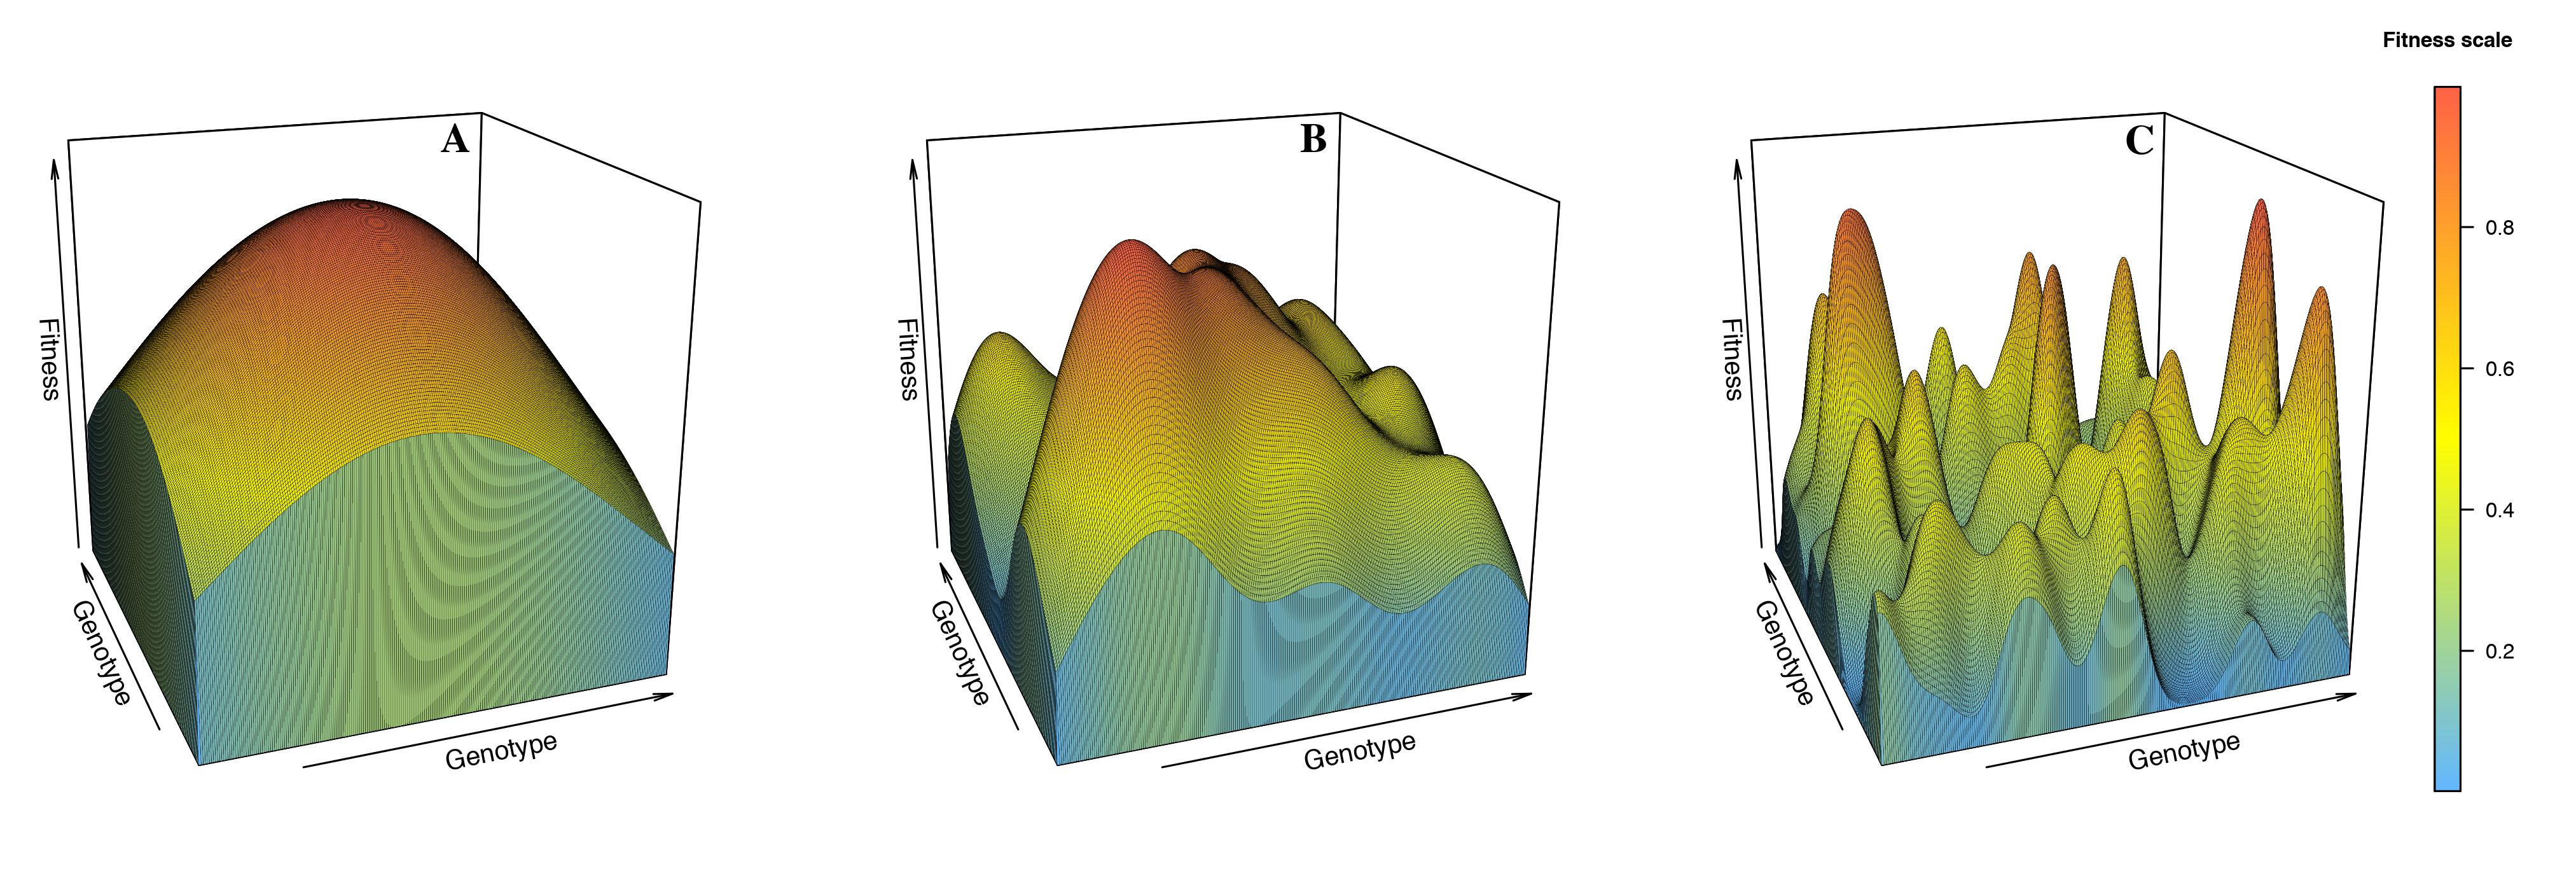
\includegraphics[scale=0.455,trim=0cm 0cm 0cm 0cm,clip]{pics/Epistasis/RuggedLandscapes.jpeg}
    \captionof{figure}{Illustration of the influence of complexity in NK models. When complexity is low ($K\approx 1$), the fitness landscape is smooth (A). Increasing K (toward the right) goes along with an increase in ruggedness of the landscape, which suggests that organisms can be trapped at local optimum - for instance in (C).}
    \label{fig:NKModel}
    \end{center}
\end{mybox}

%\begin{tabular}{ | c |}
\begin{mybox}{\begin{Note-box}
\label{Box-FisherModel}A brief description of Fisher's geometrical model\end{Note-box}}
\onehalfspacing
%\begin{minipage}{0.95\textwidth}
In Fisher's geometrical model, a phenotype is described by a set of $t$ idealized traits, each being independent from one another so that they are to be optimized specifically \citep{Fisher30} (see A below, in Figure \ref{fig:FisherModel}). These traits can consequently be depicted as independent axes in the euclidean space of the relevant dimensionality, such that fitness isoclines are represented by hyperspheres of dimension $t$ \citep{Tenaillon14}. Phenotypes are subject to stabilizing selection towards an optimum: the more an organism approaches the optimum, the lower the selective pressure is. %If an organism is fit for all but one trait, it can still be far away from the optimum since the fitness stems from the euclidean distance $d_t$ to the optimum.
\citet{Fisher30} used this model to set the stage for quantitative genetics by showing that it is more efficient to rely on a large amount of loci with small effects than the opposite as small mutational hyperspheres display very few bias towards deleterious mutations on the contrary to large ones (see B below). (Global) epistasis is also an intrinsic feature of the framework (see C below for details).
\begin{center}
    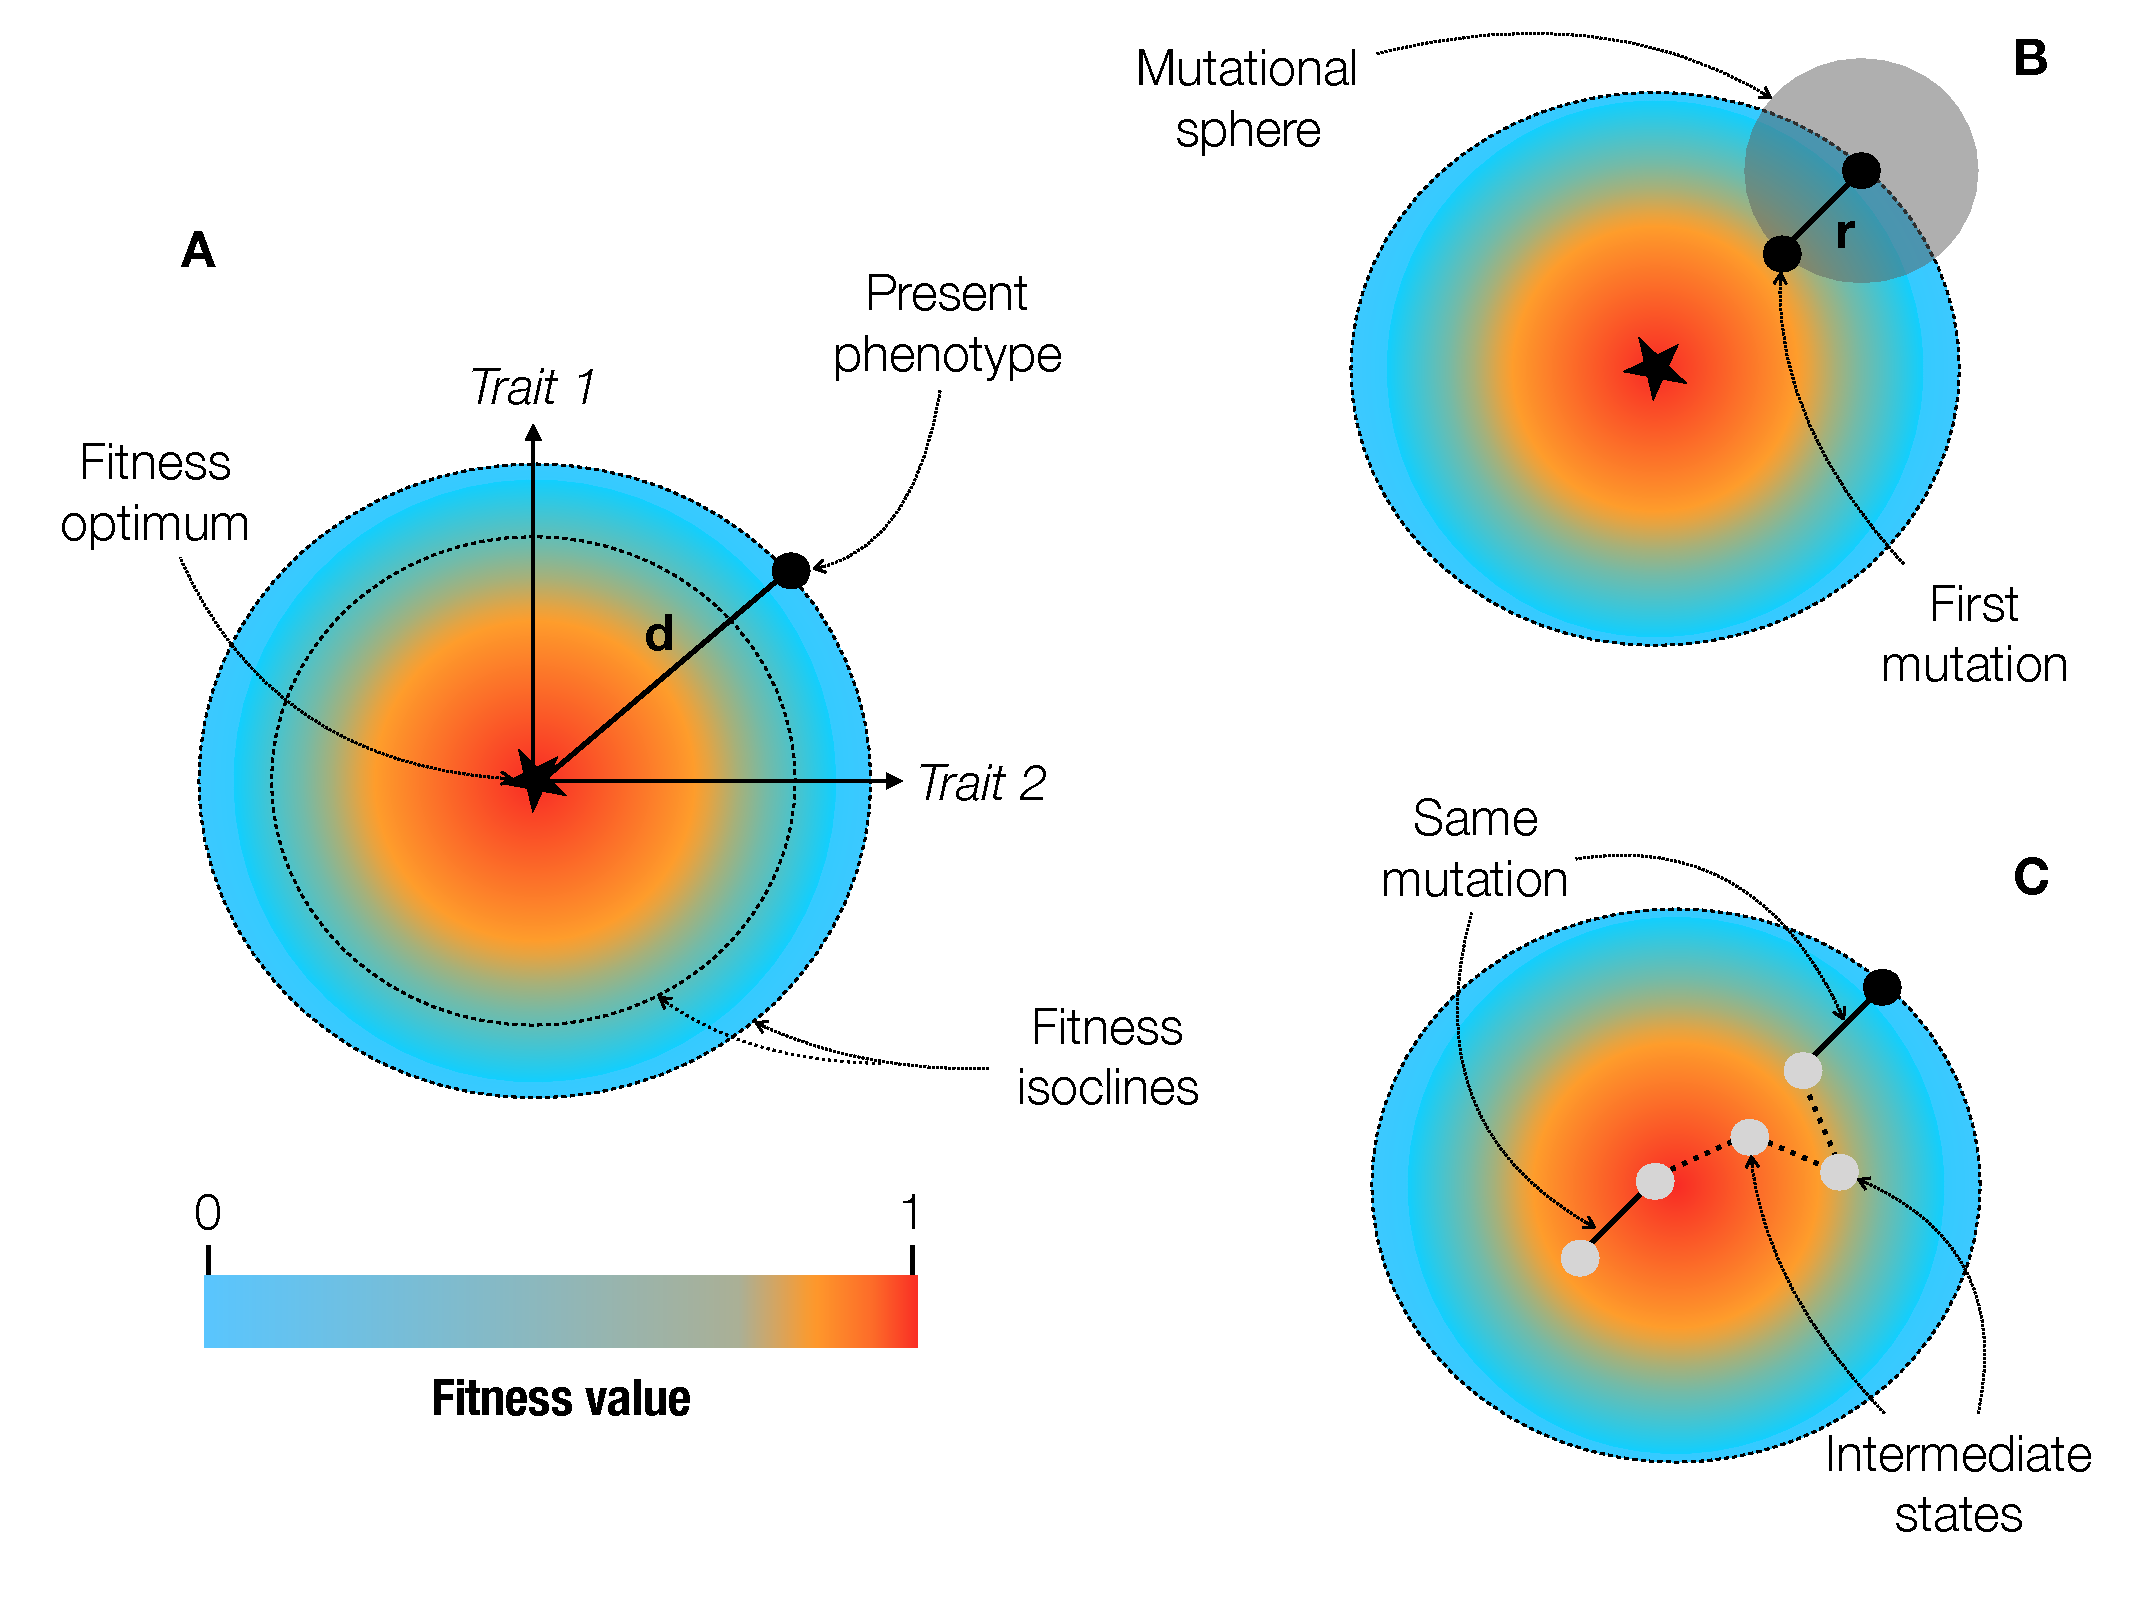
\includegraphics[scale=0.385,trim=0cm 0cm 0cm 0cm,clip]{pics/Epistasis/Fisher-Model.pdf}
    \captionof{figure}{Illustrating the framework with the two dimensional isotropic Fisher's geometrical model. The 2D fitness landscape can be described by a circle whose center represents the optimum under stabilizing selection - denoted by the star - and is surrounded by concentric fitness isoclines. This is because fitness decreases identically along any axis in the isotropic instance of the model. As shown in (B), mutations are also considered isotropic and can be represented by a sphere of radius $r$: the larger this sphere, the larger the disequilibrium between advantageous mutations (grey blue area in (B) where the two spheres overlap) and deleterious ones (grey area in (B) where mutations pull organisms further from the optimum). (C) shows that mutations with exactly similar effects on a trait may have very different impacts on fitness depending on the position in the phenotypic space : epistasis is thereby built from the core assumptions of the model \citep{Hwang17}.}
    \label{fig:FisherModel}
    \end{center}
%\begin{figure}[h]
    %\centering
    %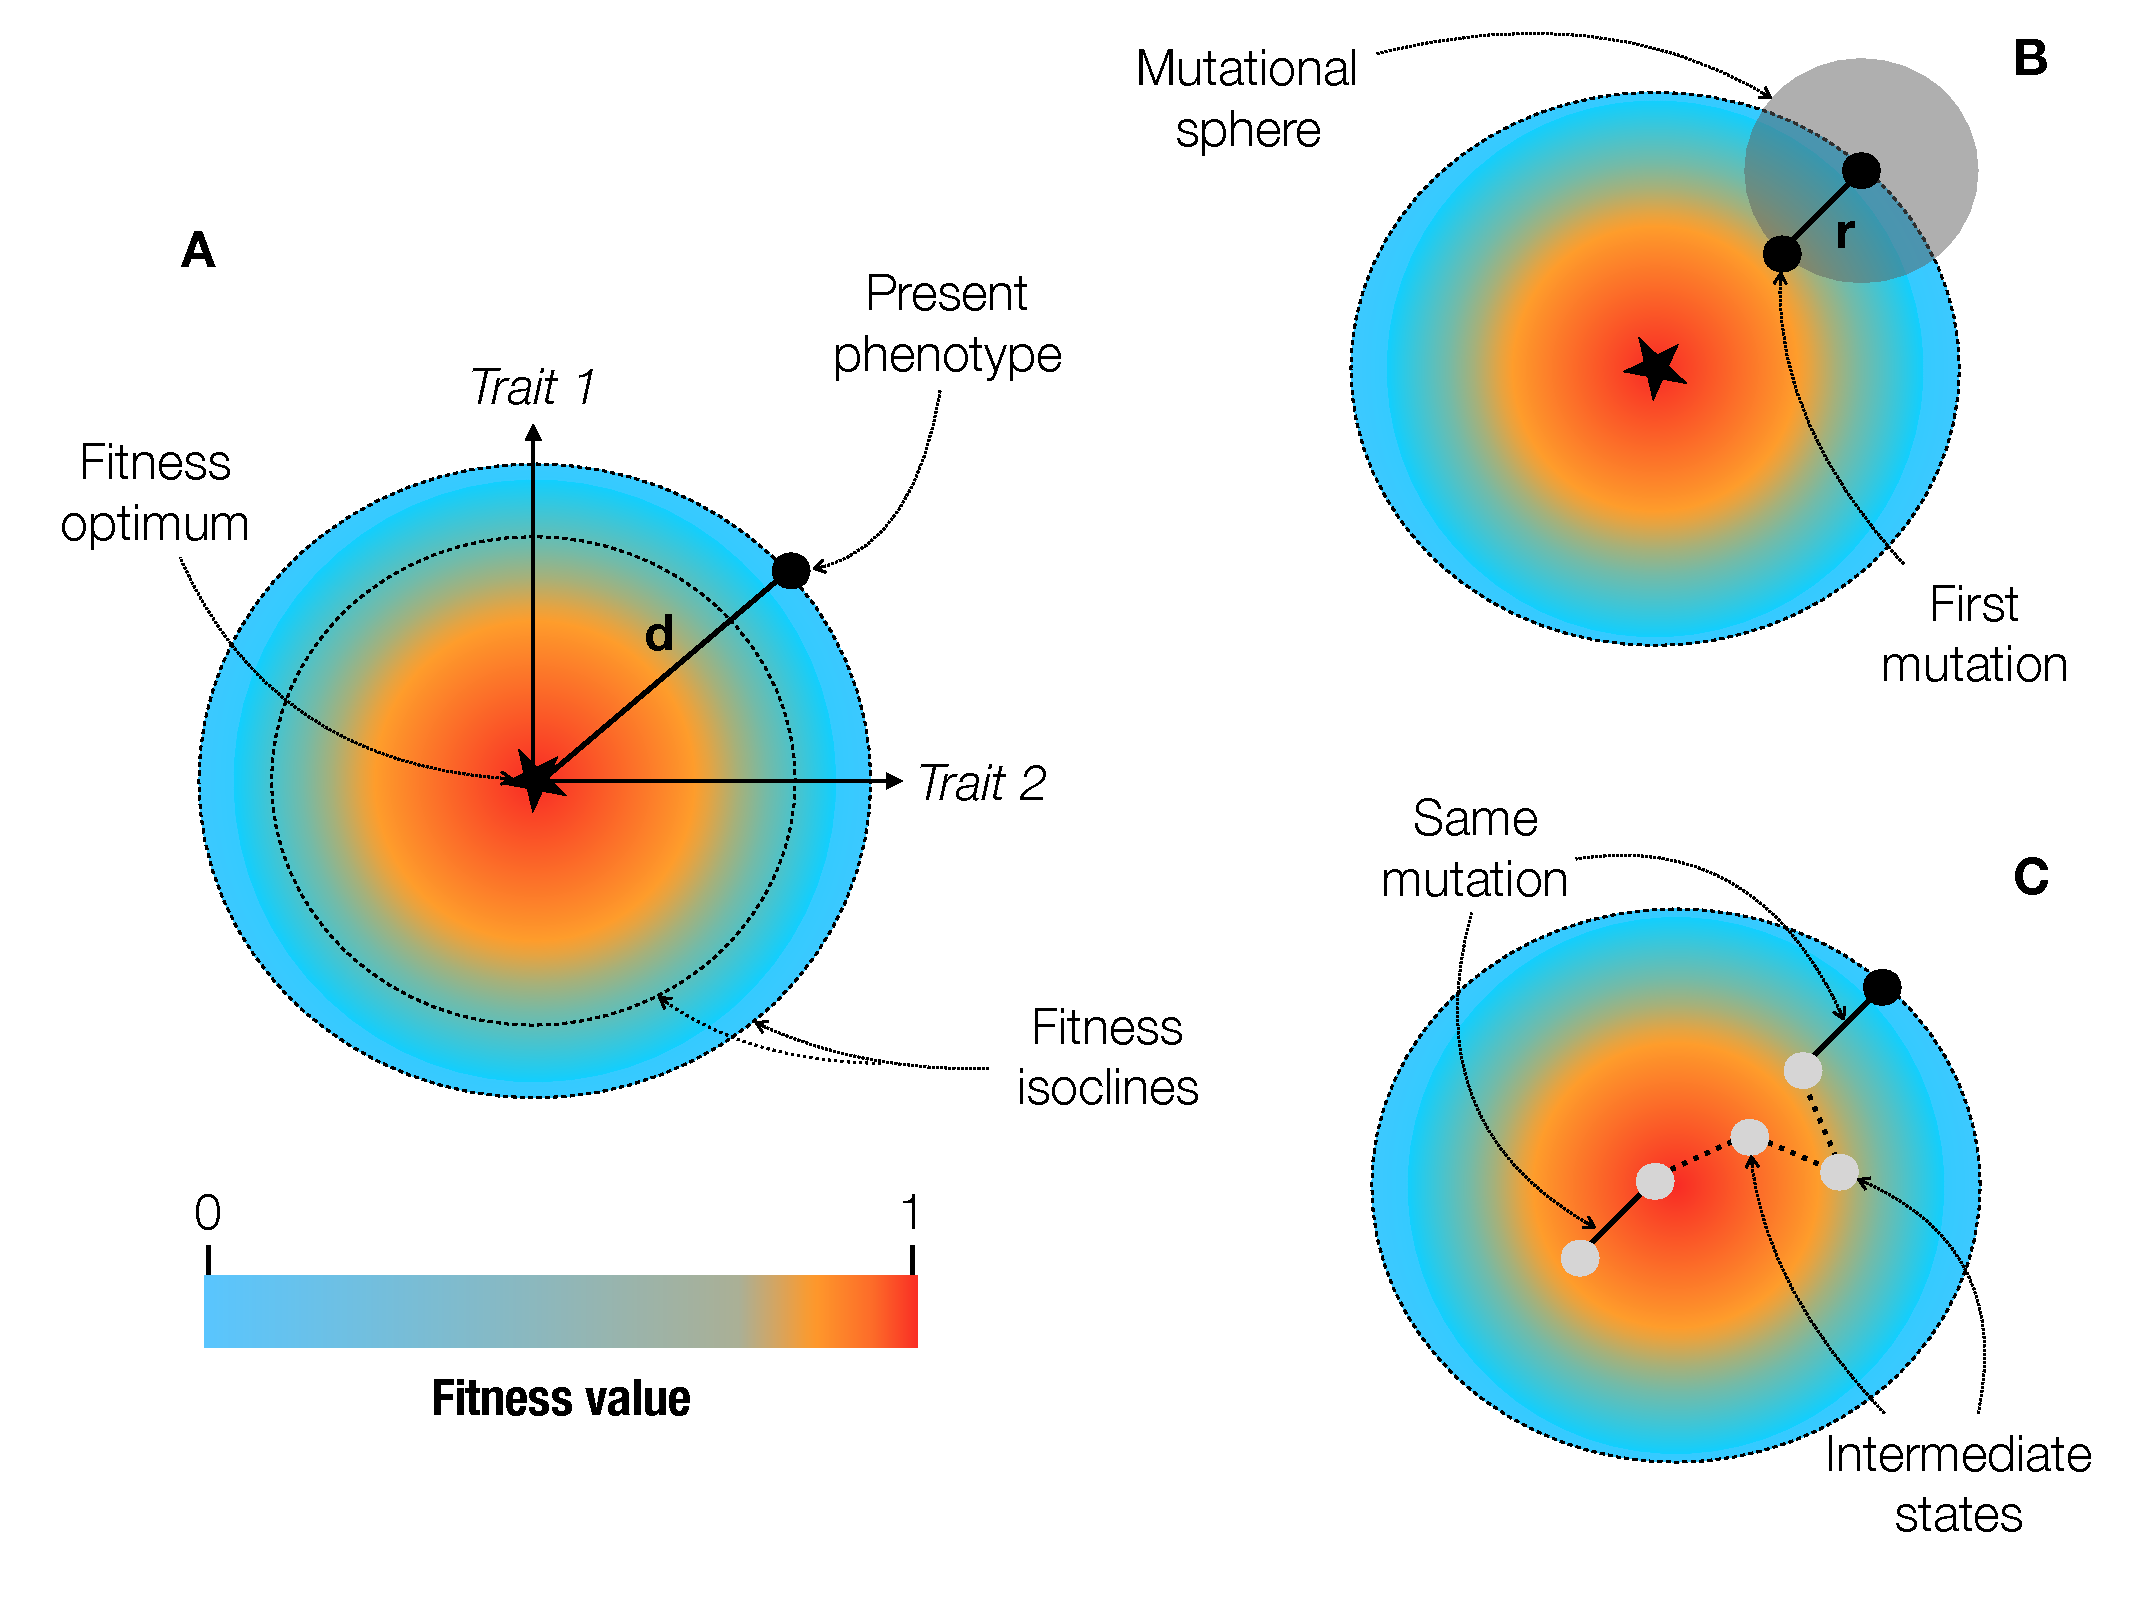
\includegraphics[scale=0.45,trim=0cm 0cm 0cm 0cm,clip]{pics/Epistasis/Fisher-Model.pdf}
    
%\end{figure}
%\end{minipage}
\end{mybox}


%\end{tabular}


\subsubsection{Putting forward the concept of high order complementary epistasis}

\begin{figure}[h!]
    \centering
    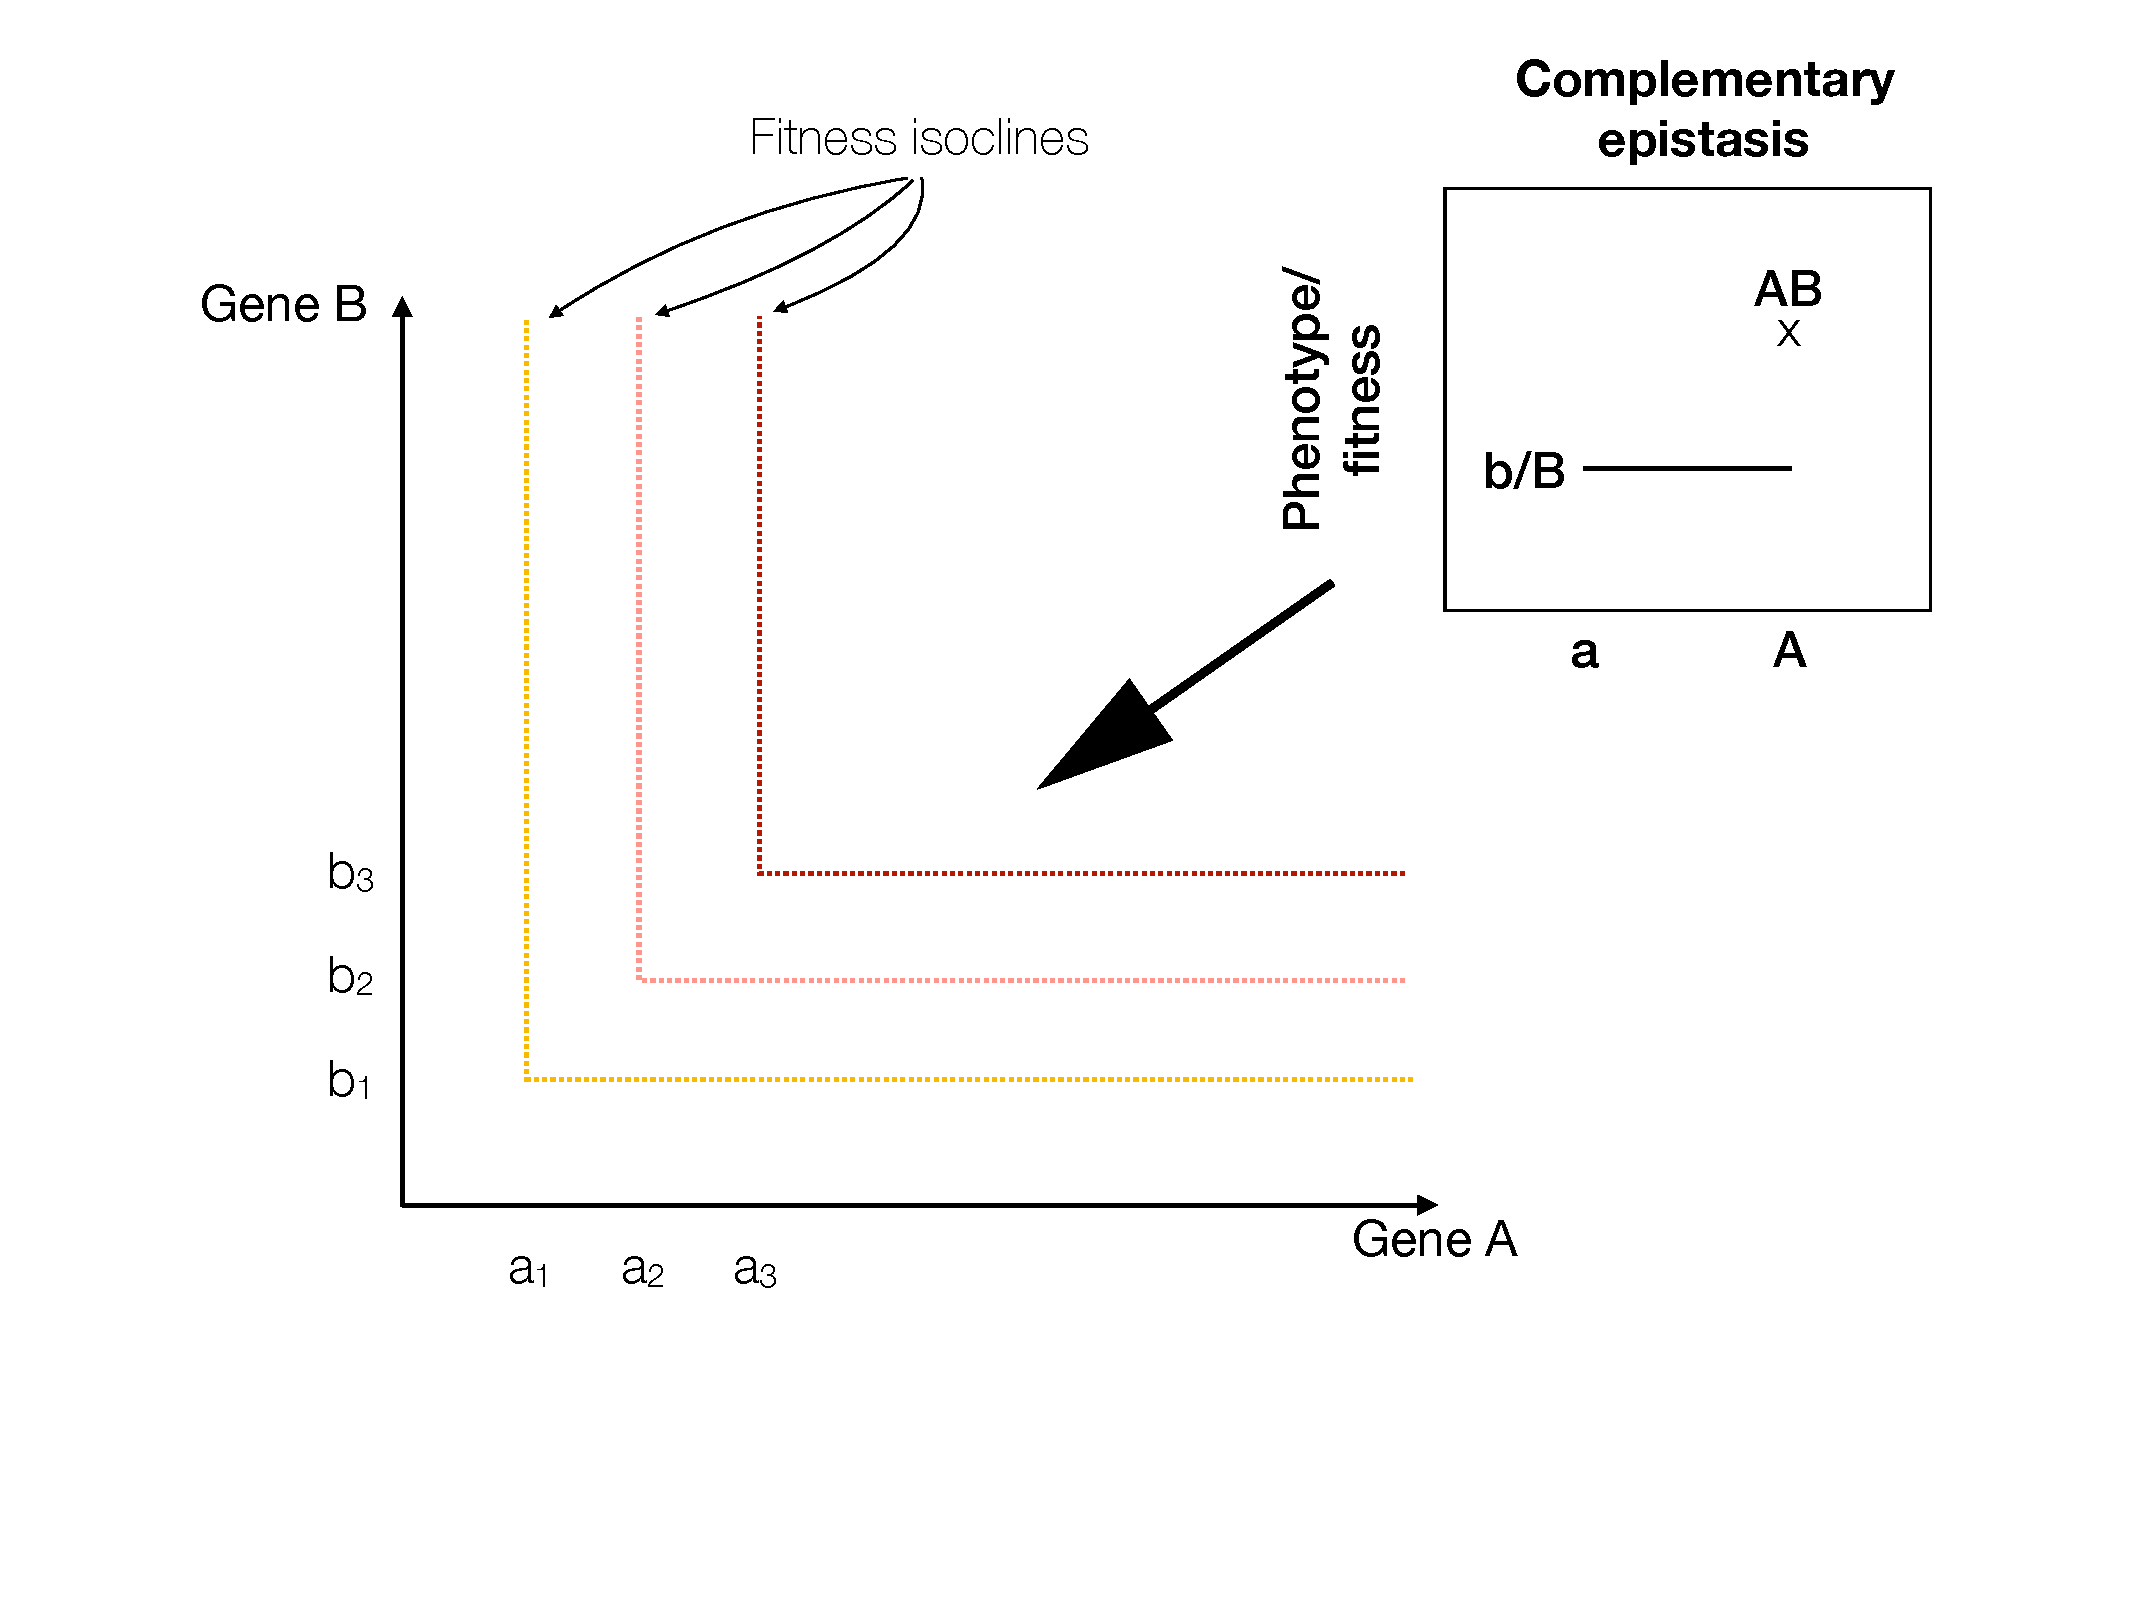
\includegraphics[scale=0.285,trim=3.2cm 4cm 3.2cm 1cm,clip]{pics/Epistasis/Complementary epistasis.pdf}
    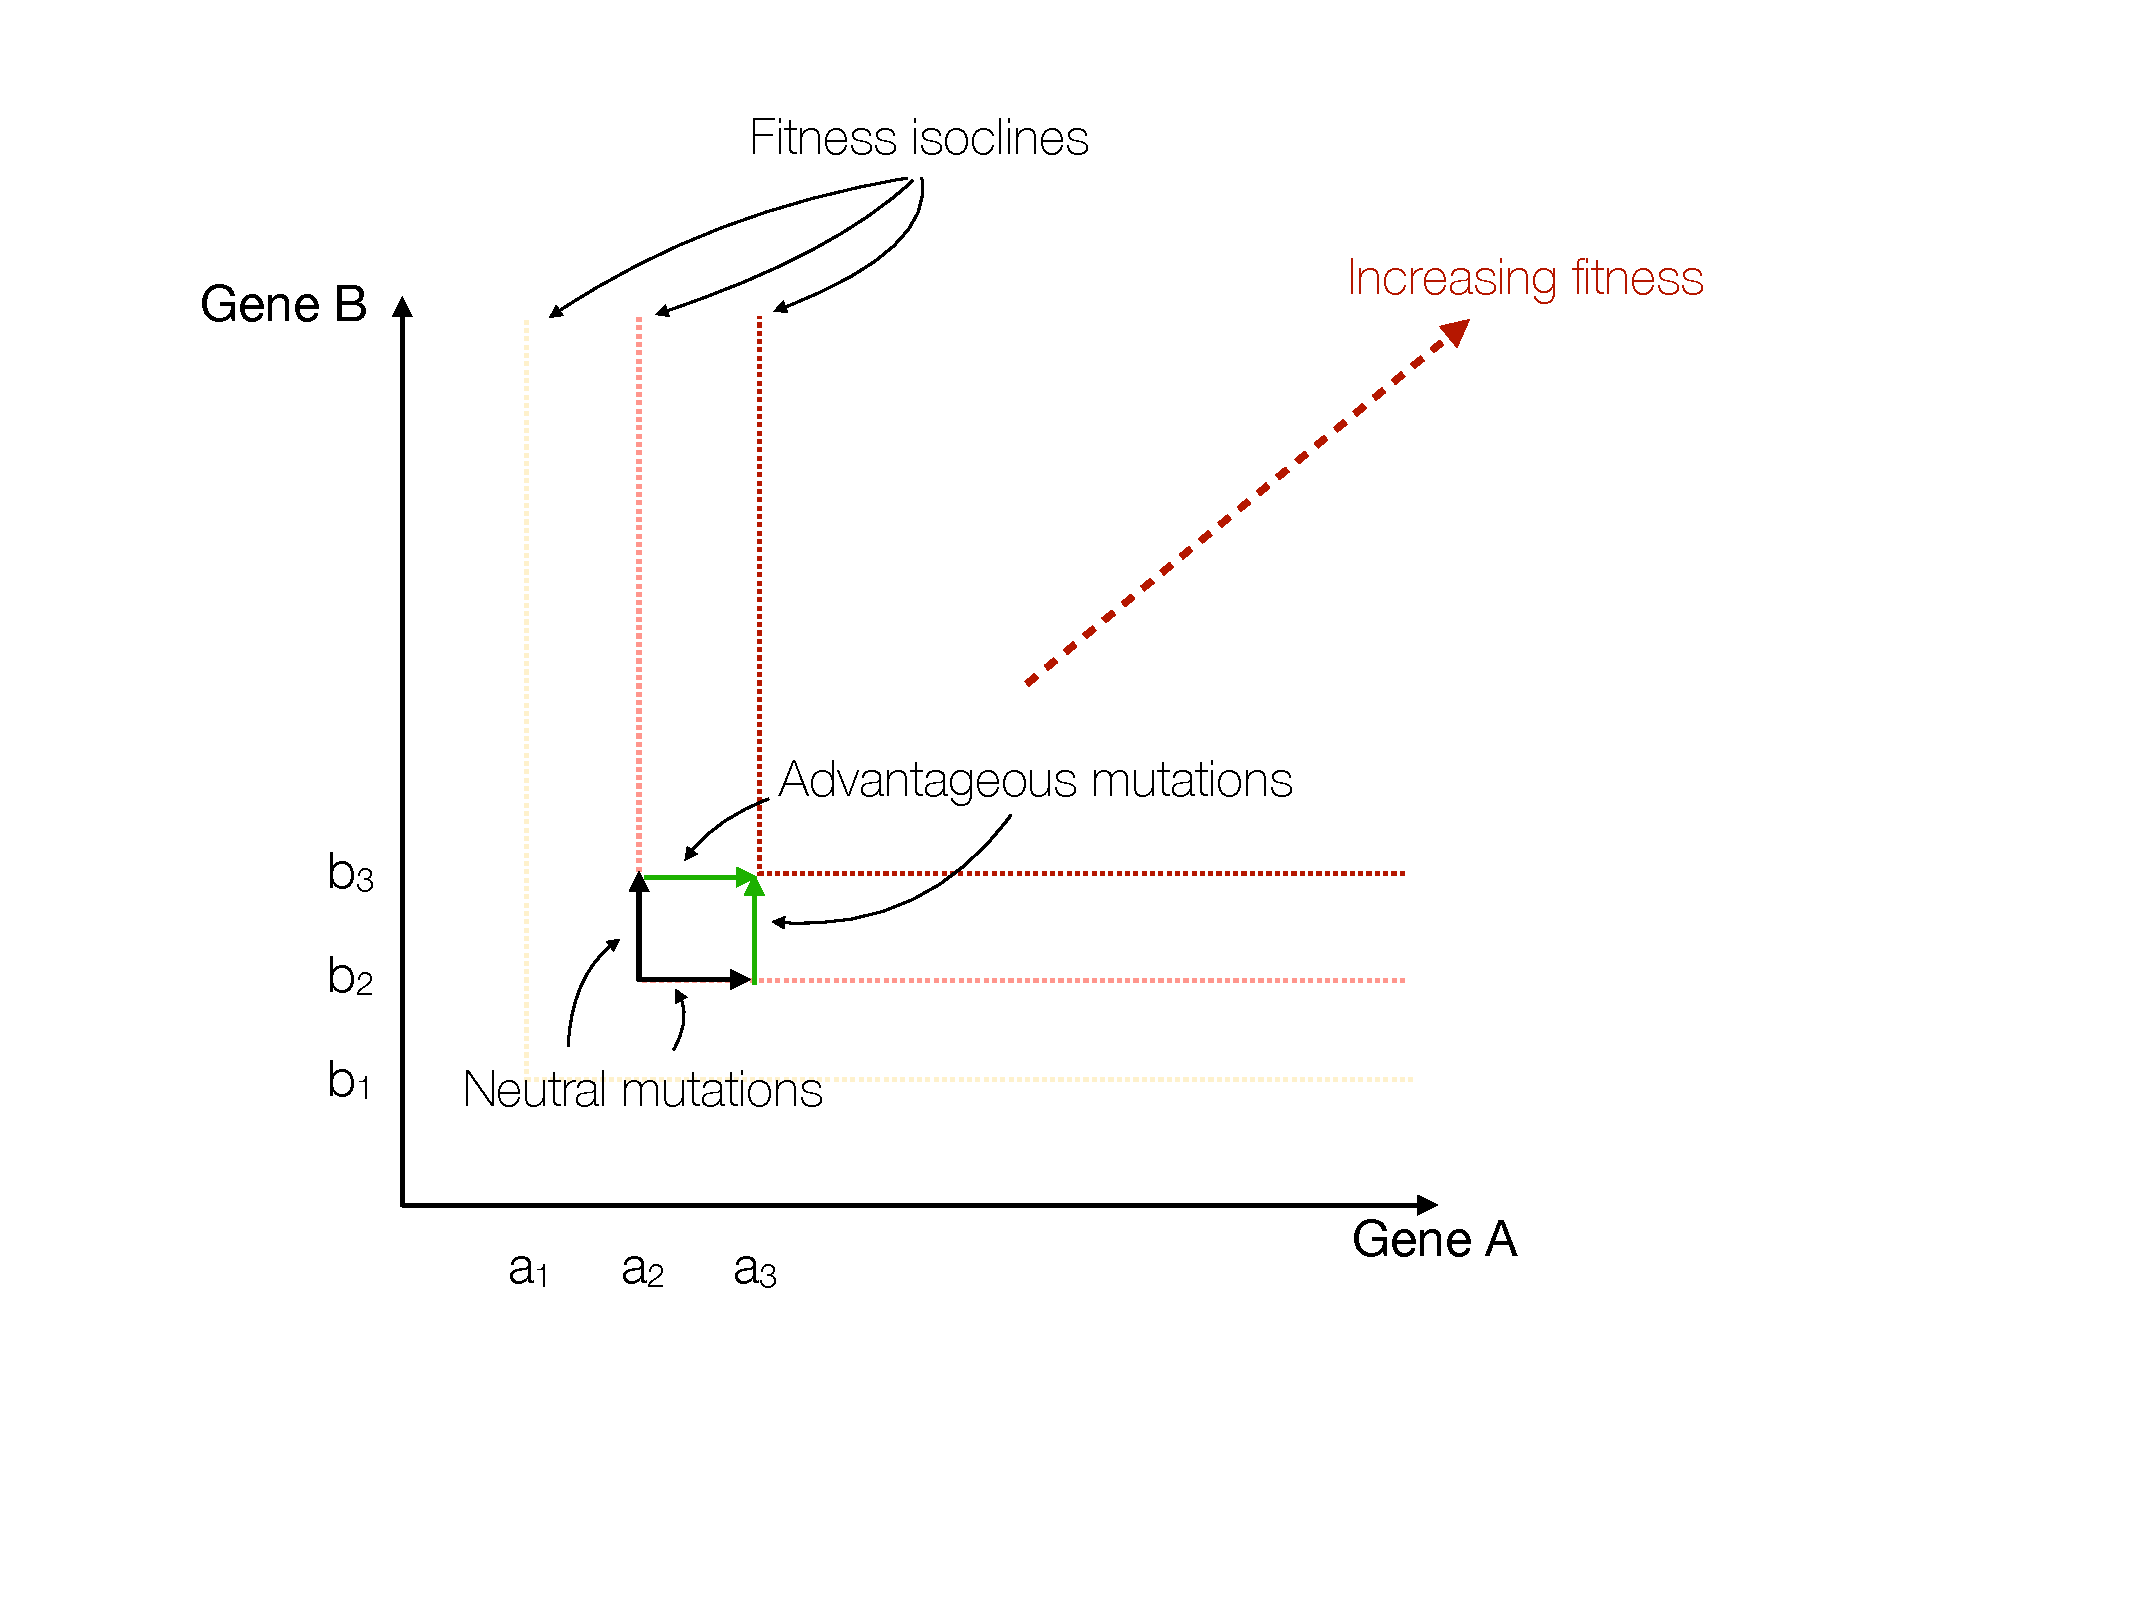
\includegraphics[scale=0.285,trim=3.2cm 4cm 6cm 1cm,clip]{pics/Epistasis/Complementary epistasis_EvoTraj.pdf}
    \caption{Description of complementary epistasis: on the left panel, its effect in the classical a/A-b/B case is shown in the short window, with the need for both A and B mutations to experience any gain of fitness, while the larger plot represents how phenotype/fitness isoclines can be mapped in the genotype space when more mutations are considered. On the right panel is also shown the mutational path that allows to gain extra fitness: first, a potentially advantageous but actually perfectly neutral mutation needs - at least - to exist on either one of the locus before the advantageous mutation can occur and give an actual extra push of fitness. This phenomenon can involve higher order interactions leading to the need for the segregation of numerous neutral mutations, which may besides be subject to mutational biases.}
    \label{fig:ComplementaryEpi}
\end{figure}

Be that as it may, it has not yet been determined how the combination of complementary epistasis \citep{Crow71,Sackton16} -- where a phenotypic trait can only be competitive if each and any of its underlying loci are (see Figure \ref{fig:ComplementaryEpi} for more details) -- with global epistasis \citep{Otwinowski18} could specifically change population genetics predictions arising from the Neutral Theory of Evolution and its extensions \citep{Kimura68,Ohta73,Ohta92} while this process seems to be to be strongly supported by mechanistic underpinnings \citep{Kacser73,Hartl85,Yi19,Taverna02,Bloom05,Labourel21} and \citet{Crutchfield00}'s work suggested that neutral diffusion in the genotype space can guide the evolution towards higher complexity\footnote{In this line of work, this neutral diffusion drives the finding of a higher complexity attraction subbasin, which gives rise to (quick) epochal evolution followed by stasis, echoing the pioneering and controversial work on punctuated equilibrium by Gould and Eldredge \citep{Eldredge71,Eldredge97}.}. This is what we propose to do in what follows; to justify the interest of such an investigation and its consequences, we start with the presentation of a toy model based on simplistic assumptions from global epistasis. We then put forward an analytical treatment dealing with a simple instance of the process. Finally, we show how this framework may have a profound impact on our understanding of Evolution at different levels of biological organization and put forward the key components that a more complete instance of the model should include. %In Perspectives & Conclusion Finally, we introduce how it can be tested and applied by contrasting its results to those obtained when simulating enzyme evolution along one and/or multiple pathways, and conclude by discussing possible further developments, among which the link with protein stability and evolutionary rates are of particular interest as well as the influence of stochastic environments on the actual coefficient of selection.

\subsection{{A first approach}\label{sec:FA}}
\subsubsection{A simplistic prediction of classical population genetics }

We expect that complementary epistasis should influence both the speed of adaptation, as was observed for evolutionary escape \citep{Weinreich05,Weissman09} and the mutational load (see introduction for previous approaches on this idea), and focus here on this latter phenomenon. More particularly, we assume that fitness should decrease with the number of units/loci involved and that the mutational bias should play a major part in hampering Adaptation because it influences the preexistence of potential complementary beneficial mutations (at loci which are drifting because they differ from the worst one). Nevertheless, it should be possible to derive a rough prediction from the underlying premises of such a phenomenon.

Based on results of the neutral theory of Evolution \citep{Kimura62,Ohta73}, we indeed know that Natural Selection cannot screen mutations whose selective effect $|s|$ is below $1/N_e$ for haploid populations. If fitness is limited by a maximum value, this means that deleterious mutations with effects $|s|\approx 1/N_e$ evolve through genetic drift and that fitness at the mutation-selection-drift balance establishes around $\prec f_1^* \succ~\approx 1-1/N_e$ when mutations are mostly deleterious and one locus is considered \citep{Kimura58}. Let us say that an organism starts with the maximum possible fitness. Through drift on the first gene, $f$ should decrease on average to approximately $1-1/N_e$. Drift on the second gene should again push fitness downwards since the maximum fitness relatively to which drift occurs is now set to $1-1/N_e$, such that $\prec{f_2^*}\succ ~\approx (1-1/N_e)\times (1-1/N_e)=(1-1/N_e)^2$. Therefore, considering $n$ complementary genes yield the following prediction $\prec{f_n^*}\succ ~\approx (1-1/N_e)^n$. If $N_e>>n$, this can be summarized by $\prec{f_n^*}\succ ~\approx 1-L^*$ using the first order Taylor expansion, with $L^*=n/N_e$ denoting the mutational load. In that case, this rough estimate is comparable in size to that from the Fisher's geometrical model in a N-dimensional space -- namely $L^*\approx n/(n+2N_e)$ -- \citep{Hartl96,Poon00,Sella09} that considers the influence of complexity on the evolutionary balance.%through patterns of pleiotropy and epistasis emerging from the underlying assumptions of the model \citep{Tenaillon14}.

\subsubsection{A toy evolutionary model}

In this toy model, we consider a fitness landscape subject to saturation due to diminishing returns epistasis \citep{Tokuriki12,Kaltenbach14} as has widely been documented for proteins in the case of stability \citep{Taverna02,Bloom05,Bloom06,Kaltenbach14} and catalytic efficiency \citep{Dykhuizen87,Hartl85,Yi19,Labourel21}. It has also been recently shown that global diminishing returns epistasis \citep{Kryazhimskiy14,Bahcall14,Otwinowski18} should arise for a complex trait as a by-product of the distribution of fitness effects \citep{Reddy20}. Such a fitness landscape can typically be described through a sigmoid function whose shape is given by the following equation (similar to that of Michaelis Menten):
\begin{align}
    f(x)=\frac{x}{x+K_X}
    \label{eq_sat}
\end{align}
The evolutionary process is then simulated using the probability of fixation \citep{McCandlish14}, which is a classical result in population genetics \citep{Haldane27,Kimura62,Wright31}. Within this simplified framework, neither clonal interference nor double/multiple mutants are considered, meaning that the fixation process concerns only one mutation (on one gene) at a time through a pairwise competition. Under this assumption, the probability that a mutation occurring in a haploid population is eventually fixed is given by:
\begin{align}
    P_{\text{fix}}(s,N_e)=\frac{1-e^{-2s}}{1-e^{-2N_es}}(\approx \frac{2s}{1-e^{-2N_es}} \text{, when $s<<1$})
\end{align}
 Let us say that $\mathbf{X}=(X_1,...,X_n)$ is the vector representing a state of the pool of $n$ complementary gene\footnote{For convenience, we only mention genes, but as stated previously, it may also apply to loci or organismic units, for instance.} where  $X_i$ denotes the phenotypic value of the $i^{eth}$ gene, and that $s_m'=\frac{f(X_m')-f(X_m)}{f(X_m)}$ denotes the potential selective value of a mutation $X_m'$ with fitness $f(X_m')$ occurring on the gene $m$ whose current value in the population is $X_m$ (and fitness $f(X_m)$). The fitness function detailed above therefore determines the maximum fitness a gene can potentially induce (\textit{e.g.} the maximum catalytic flux an enzyme may be able to sustain without incurring costs). The actual selective value of a mutation, and its evolutionary fate, depends on the whole genetic background $\mathbf{X}$ within which it occurs owing to the specific process of complementary epistasis that changes the selective effect this mutation provides to its carrier. Two cases have to be distinguished, as we specified below and on Figure \ref{fig:CompEpi-FixProb}.
 
 First, if the mutation affects the less efficient gene of a pool of complementary genes -- \textit{i.e.} $X_{m}=\min \limits_{i \in S_g} (\mathbf{X})$, such that $f_{\mathbf{X}}=f(X_m)$, with $S_g$ the set of genes involved in the phenotypic set $\mathbf{X}$ -- the probability of fixation of the mutation $X_m'$ rises only up to the threshold where it is no longer the worst gene among the pool. It yields:
 \begin{align}
     P_{\text{fix},X_{m}'} = \left\{
    \begin{array}{ll}
        P_{\text{fix}}(s_m',N_e)\text{, when $s_m'$} \leq \Delta s_{\{m,max\}} \\
        P_{\text{fix}}(\Delta s_{\{m,max\}},N_e)\text{, otherwise,}
    \end{array}
\right.
\label{eq:Pfix_compepi1}
 \end{align}
 
where $\Delta s_{\{m,max\}}=\min \limits_{\substack{i \in S_g \\ i\neq m}} \frac{f(X_i)}{f(X_m)} - 1$ (with $\Delta s_{\{m,max\}} \geq 0$). 

Conversely, if the mutation influences the phenotypic value of any other gene -- \textit{i.e.} $X_{m}>\min \limits_{i \in S_g} (\mathbf{X})$, with $S_g$ the set of genes involved in the phenotype $\mathbf{X}$ -- its probability of fixation is that of a perfectly neutral mutation as long as the phenotypic value for this gene remains above the minimum of the set while it is that of a disadvantageous mutation -- relatively to this threshold -- when it falls under it, such that:
 \begin{align}
     P_{\text{fix},X_{m}'} = \left\{
    \begin{array}{ll}
        1/N_e\text{, when $s_m'$} \geq \Delta s_{\{m,min\}} \\
        P_{\text{fix}}(s_{\{act,m'\}},N_e)\text{, otherwise,}
    \end{array}
\right.
\label{eq:Pfix_compepi2}
 \end{align}
 
where $\Delta s_{\{m,min\}}=\min \limits_{\substack{i \in S_g}} \frac{f(X_i)}{f(X_m)} - 1$ (with $\Delta s_{\{m,min\}} \leq 0$) and $s_{\{act,m'\}}=\frac{f(X_m')}{\min \limits_{\substack{i \in S_g}} f(X_i)}-1$.\\

\begin{figure}[h!]
    \centering
    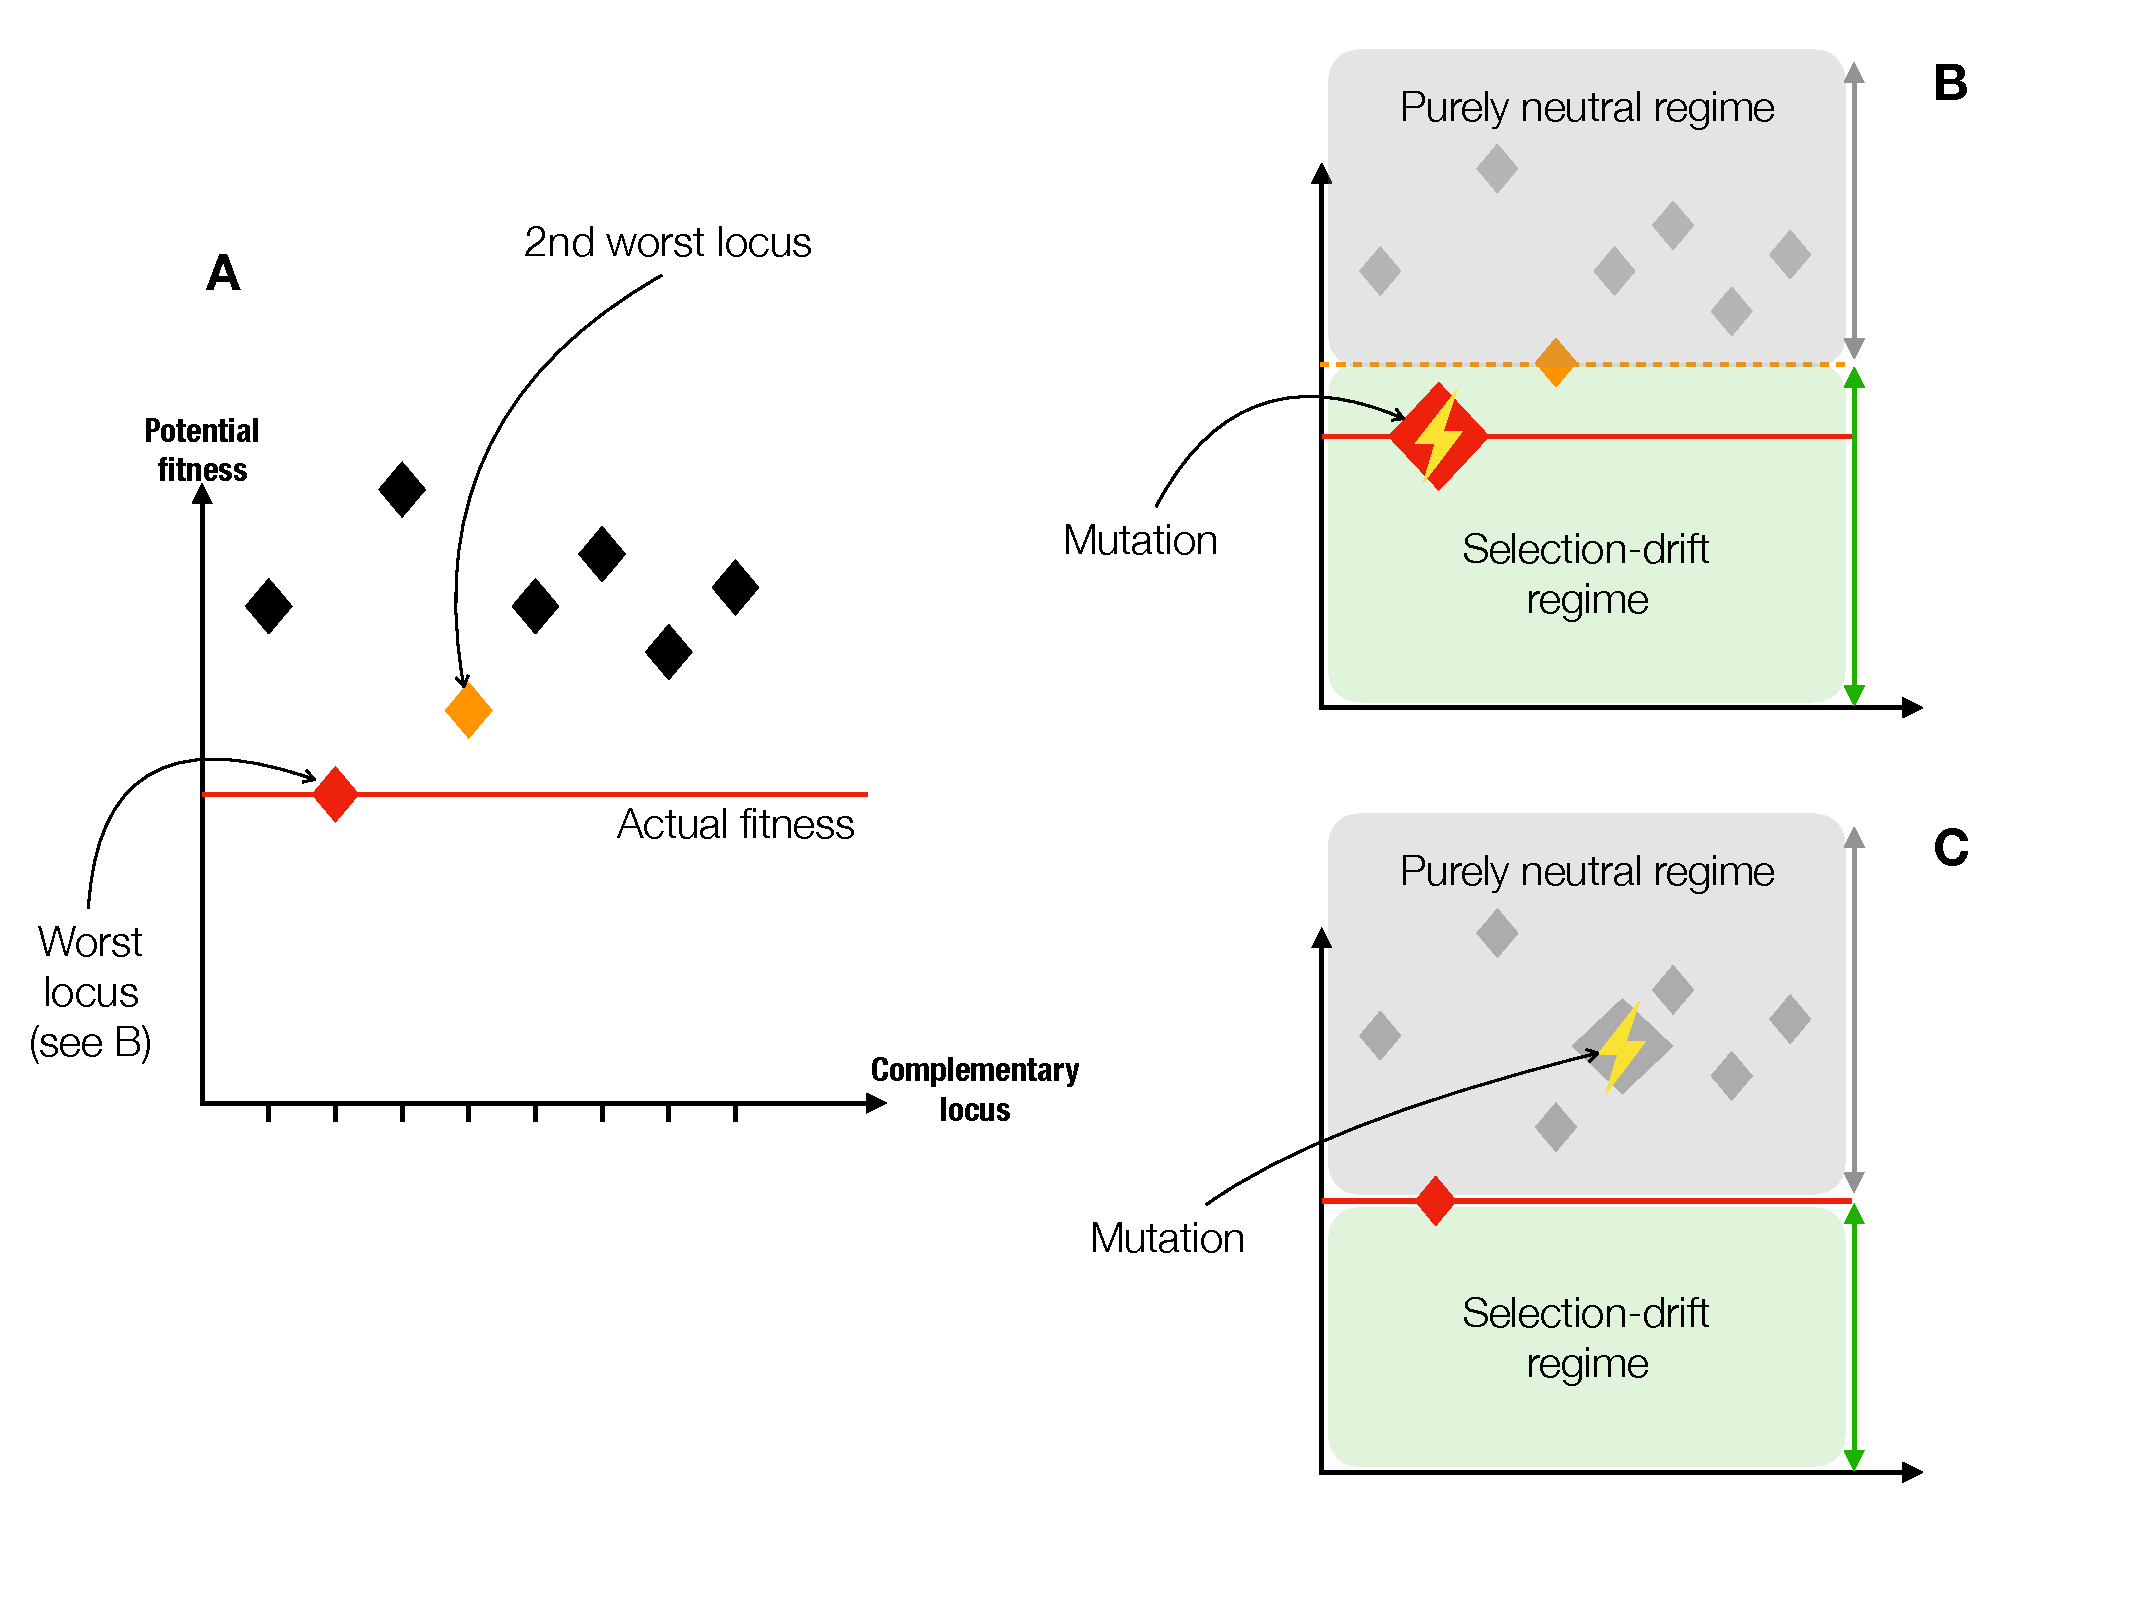
\includegraphics[scale=0.45,trim=0cm 1cm 0cm 1cm,clip]{pics/Epistasis/Selection-Complementary-Epistasis.pdf}
    \caption{Explanations on how the probability of fixation depends on the locus affected by a mutation: as shown in A, the actual fitness is determined by the potential fitness of the worst locus. In accordance with that, two cases are to be distinguished : if the mutation hits the worst one (B), it evolves under selection-drift regime (with $P_{fix}$ corresponding to the single locus model expectation) up until its potential fitness reaches the $2^{nd}$ worst one of the set of complementary loci, where any extra improvement would have the same selective value as that provided by the difference between the two worst loci; on the other hand, if the mutation hits one of the other (then the worst one) loci, it evolves under pure neutrality ($P_{fix}=1/N_e$ for haploid Wright-Fisher process) down to the actual fitness because it does not affect this latter, and it is only below this threshold that it can be counter-selected according to the drift-selection regime.}
    \label{fig:CompEpi-FixProb}
\end{figure}

We considered the influence of different distribution of fitness effects by drawing phenotypic values $X_m'$ according to the following equation :
\begin{align}
\log_{10}(X_m') \sim \mathcal{N}(\log_{10}(X_m)-b,\sigma_X),
\end{align}
where $b$ represents the intensity of the bias towards deleterious mutations. To comply with estimates on biological phenotypic traits, be they catalytic constants \citep{Carlin16} or gene expression \citep{Metzger16,Hodgins-Davis19}, the distribution of mutational phenotypic effects is modelled through a Gaussian distribution whose mean depends on the present value of the trait $X_m$ at the loci $m$ and a variance $\sigma_X^2$ (and the aformentionned mutational bias). We examined different situations ranging from cases where no mutational bias exists ($b=0$) to some with high ones ($|b|=\lambda X_m$, where $\lambda>>0$). Both because it seems more realistic \citep{Carlin16} and because the optimization process would otherwise be far longer, mutations are drawn for the $log_{10}$ value of the trait in such a way that those affecting higher phenotypic values have a proportionally higher variability and are more biased (when the bias is not null).

Note that there exists a broad scientific literature on the distribution of fitness effects of mutations \citep{Keightley07,Orr03,Gillespie84} and some previous theoretical arguments for it (see for instance \cite{Martin06} and \cite{Rice15}), but we are here interested in the making of these effects from underlying causes and cannot, as a consequence, use distributions that result from evolved phenotype-fitness maps. We shall later discuss this point as a direct perspective of the present project.

\subsubsection{Simulation results}

As an attempt to evaluate the relevance of studying this phenomenon, we tested as a premise the influence of complementary epistasis on the mutational load. To do so, we set $K_X=1$ in equation (\ref{eq_sat}). Three mutational biases were considered ($0$;$-\sigma_X$;$-2\sigma_X$) ranging from no bias to a high one through which only 1 mutations out of 40, approximately, is advantageous. We also studied two different levels of phenotypic variability among mutants for the $log_{10}$ of $X_m'$ ($\sigma_X=0.25$ and $\sigma_X=0.5$), with the highest one producing advantageous mutations with greater selective effects while decreasing the relative pool of slightly deleterious ones. These sets of parameters are in line with the aforementioned estimates for some distribution of phenotypic effects of mutations \citep{Carlin16,Metzger16}. The initial value of each complementary phenotypic trait was set to $X_i=X_0$ for any gene, with $X_0=1-1/N_e$ to start from the null hypothesis of nearly-neutral Evolution under high deleterious bias (but only one module). This starting point thus coincides with the classical Wright and Kimura's expectation and should outstrip the final value as any extra epistasis comes at a cost. Finally, the probability of fixation was computed through either equation (\ref{eq:Pfix_compepi1}) or equation (\ref{eq:Pfix_compepi2}) depending on the locus which was affected and the simulations were ran for an average of $10
^3$ mutation events per gene per ideal Wright-Fisher individual (\textit{eg.} if $N_e=10^2$, $10^5$ mutations are drawn per gene).

\begin{figure}[h!]
    \centering
    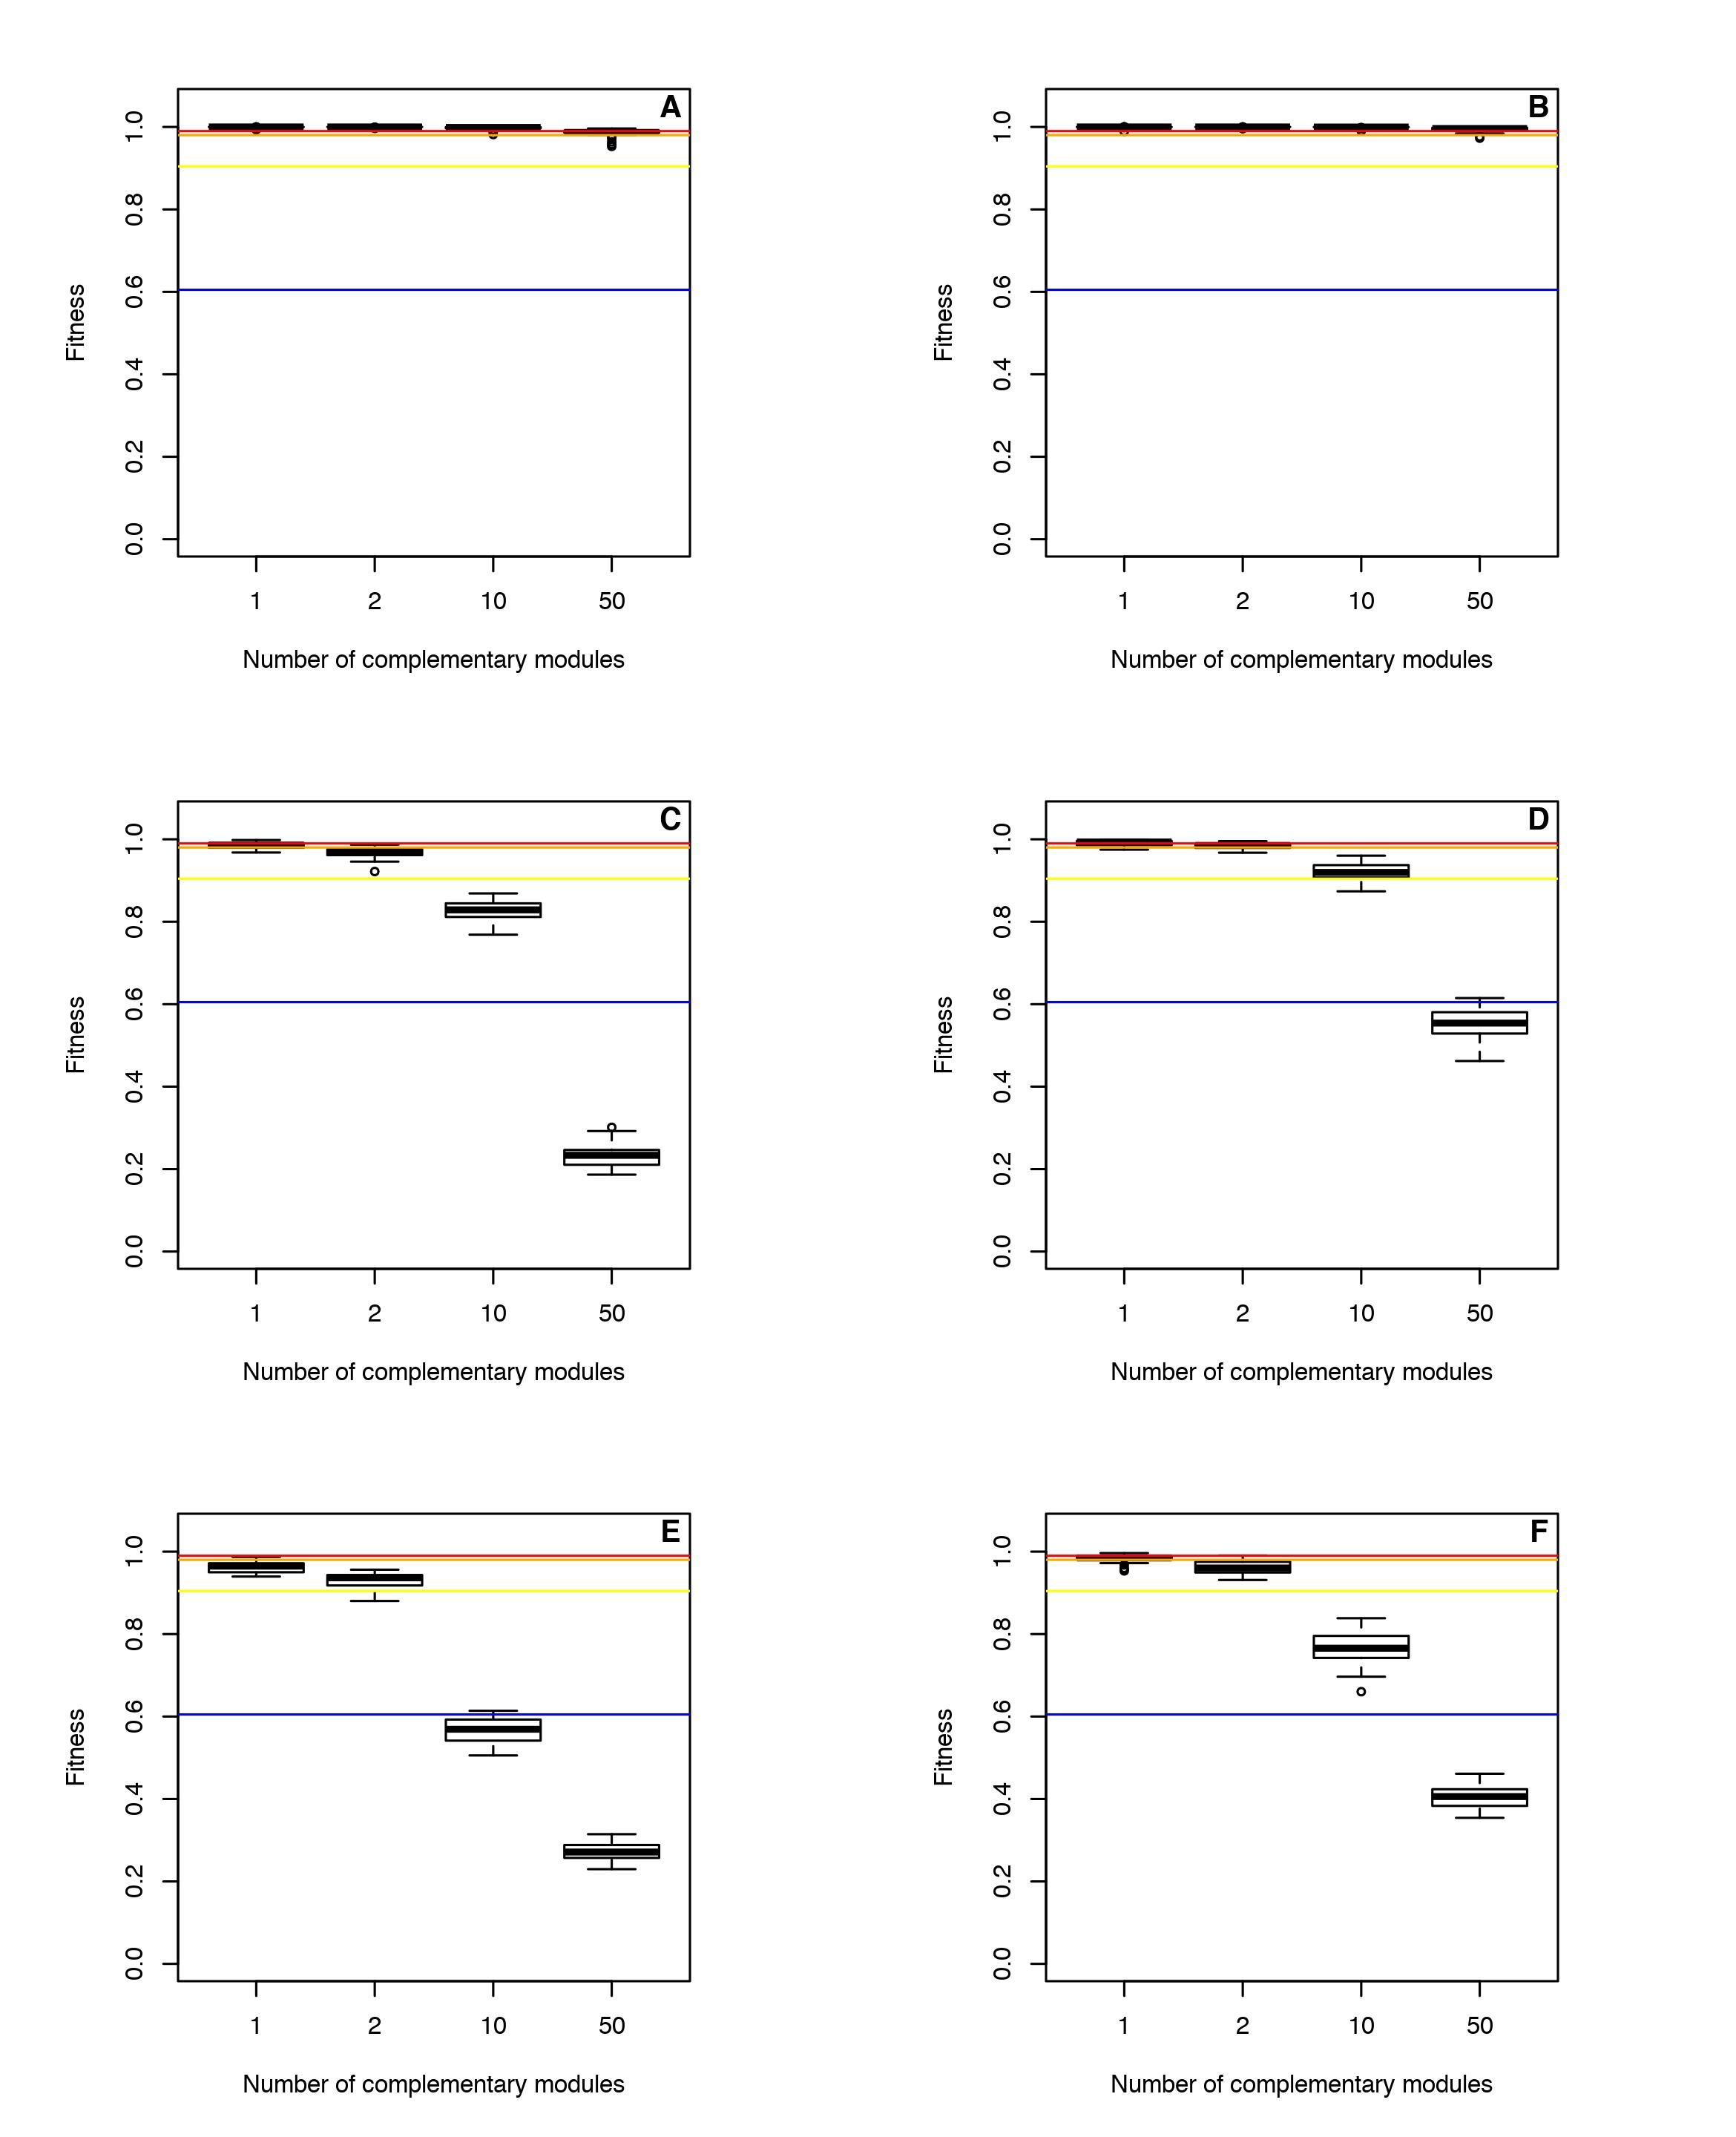
\includegraphics[scale=0.83,trim=0cm 0.4cm 0cm 0.75cm,clip]{pics/Epistasis/Evo_Outcomes_Ne100.jpeg}
    \caption{Simulation outcomes for the fitness at mutation-selection-drift balance with $N_e=10^2$ under the interplay of complementary epistasis and diminishing returns epistasis (through the fitness landscape of traits). The number of complementary modules (\textit{eg.} genes) varies from 1 to 50. Each line corresponds to a level of mutational bias: null in (A) and (B), low in (C) and (D), high in (E) and (F) - see text for details; each column represents a level of mutational variability, with (A), (C) and (E) having low variability while (B), (D) and (F) display a moderately high variability.}
    \label{fig:Outcomes100}
\end{figure}

We simulated the evolutionary process for $N_e=10$ (see Appendix section at the end of this subsection) and $N_e=100$ and present the results obtained for the mutational load in this latter case. In line with expectations, we observed that the number of complementary genes (denoted under the generic term of modules in the figure) severely impairs the strength of Natural Selection, with a decrease of the order of $n_{mod}\times 1/N_e$ when mutational biases are considered. However, this is not the case when no bias is considered with a decrease being far more limited that does not jeopardise the optimisation process albeit marginally - see (A) and (B) on Figure (\ref{fig:Outcomes100}). Because deviations from the expected steady-state can accumulate, the balance is also more sensitive to the variability of mutational effects, with lower variability coming with a predictable decreased fitness - due to an increased amount of slightly deleterious mutations and a decreased amount of largely advantageous mutations - for the same level of mutational bias (compare (C) and (E) with (D) and (F) on Figure (\ref{fig:Outcomes100})). Owing to the very low effective population sizes, drift overwhelms Natural Selection and pushes the balance towards very low values, a process already documented in models based on universal pleiotropy such as \citep{Hartl96} and \citep{Poon00}. But we show here using a toy model that such complexity-selection trade-off may be readily observed without any preexisting pleiotropic relationship (and without accounting for the decrease of effective population size usually associated with complexity), which lends credit to the idea of an intrinsic cost to complexity.

\subsection{Towards an analytical treatment ?}

In order to grasp the effect of high order complementary epistasis, it is of great interest to derive results in terms of phenotypes and fitness distributions, rather than only the mutation load it entails. Based on insights by \citep{Sella05}, who shown that assuming weak mutations - such as in Moran or Wright-Fisher model - it is possible to determine the distribution of fitness at evolutionary steady-state as a combination between the neutral distribution of fitness and the effect of the power of selection $N_e$ using the formula:
\begin{align}
 \rho^*(f)   = \frac{f^v.\rho_g(f)}{ \int_{0}^{1} f^v.\rho_g(f) \, \mathrm{d}f }, 
\end{align}

where $v$ denotes the temperature analogy and can be estimated for both Moran and Wright-Fisher models (\textit{eg.} haploid Wright-Fisher model $v=2(N_e-1)$), $f$ represents any possible value of fitness for a genotype, and $\rho_g(f)$ is the neutral distribution of fitnesses in the genotype space. In this formula, one assumes symmetrical mutations ($\mu_{ij}=\mu{ji}$), but it is possible to relax this assumption \citep{Sella05}.

For example, if fitness is uniformly distributed between 0 and 1, meaning that $\rho_g(f) \sim \mathcal{U}(0,1)$, it is straightforward to show that the steady-state distribution of fitness is given by:
\begin{align}
    \rho^*(f)   =\frac{f^v}{1/(v+1)}=(v+1)f^v
\end{align}
As a direct consequence, such a fitness distribution yields the following mutational load:
\begin{align*}
    L^*=1-\prec f^*\succ &=1- (v+1)\int_{0}^{1} f^{v+1}.\rho_g(f) \, \mathrm{d}f\\
    &=1-\frac{v+1}{v+2}\\
    &=\frac{1}{v+2}\\
    &(=\frac{1}{2N_e}\text{for an haploid Wright-Fisher population})
\end{align*}

Simultaneously, the fundamental theorem of order statistics \citep{Casella02} enables one to determine the distribution of the $k^{ieth}$ order statistic. More particularly, the distribution followed by the minimum $X_{(1)}=\min \{X_1,X_2,...,X_n\}$ of a n-tuple of random variables identically distributed obeys the following equation:
\begin{align}
    f_{X_{(1)}}(x)=n~f(x)~(1-F(x))^{n-1},
    \label{eqFO_formula}
\end{align}

where $f(x)$ and $F(x)$ respectively represents the density and cumulative probability distribution of these variables.

It is therefore possible to determine the neutral distribution of fitness using known distributions under certain circumstances. A simple didactic case corresponds to the aforementioned uniform distribution, for which it is known that the first order statistic obeys a Beta distribution $\mathcal{B}(1,n)$ when $n$ variables are drawn. The neutral distribution of fitness under complementary epistasis is therefore given by this distribution, which yields that the fitness distribution at evolutionary steady-state also follows a Beta distribution as:

\begin{align}
 \rho^*(f)   = \frac{f^v.(1-f)^{n-1}}{ \int_{0}^{1} f^v.(1-f)^{n-1} \, \mathrm{d}f },
\end{align}

Notice that the scaling factor made by the beta function vanishes as it is present on both sides of the fraction. It follows that $\rho^*(f) \sim \mathcal{B}(v+1,n)$, whose expectancy - which corresponds to fitness at mutation-selection-drift balance - is given by $\prec f^*_{\mathcal{U}_n} \succ~=\frac{v+1}{v+1+n}$, which yields $\prec f^*_{hap,\mathcal{U}_n} \succ~=\frac{2N_e-1}{2N_e-1+n}$ in an haploid population for a corresponding mutational load of $L^*_{hap,\mathcal{U}_n}=\frac{n}{n+2N_e-1}$. Remarkably, this burden is the exact same quantity than that derived from Fisher's N dimensional geometric model, meaning that the latter coincides with a model of complementary epistasis where the neutral distribution of fitness is uniformly distributed.

Nonetheless, we know that such a distribution is not very realistic. Instead, the fitness distribution is more likely to obey a Beta-like distribution whose parameters may differ on a case-by-case basis. Beta-distributions do not enable analytic tractability, but \citet{Kumaraswamy80} put forward the beta-like Kumaraswamy distribution, which allows such calculations \citep{Jones09}. This distribution is described by the following DFD:
\begin{align*}
    f(x;a,b)=abx^{a-1}(1-x^a)^{b-1} \mathds{1}_{[0,1]},
\end{align*}
for which it is possible to write the first order statistic using Eq.(\ref{eqFO_formula}) and to apply it to the fitness distribution:
\begin{align*}
    \rho_g(f)=n\times abf^{a-1}(1-f^a)^{b-1}\mathds{1}_{[0,1]} ((1-f^a)^b))^{n-1}
\end{align*}
Rearranging the terms to gather $n$ and $b$ ones, it is straightforward to show that $\rho_g(f) \sim \mathcal{K}(a,nb)$. Consequently, the distribution of fitness at evolutionary steady-state obeys the following law:

\begin{align}
    \rho^*(f)   = \frac{a(nb)f^{v+a-1}(1-f^a)^{nb-1} \mathds{1}_{[0,1]}}{\int_{0}^{1} a(nb)f^{v+a-1}(1-f^a)^{nb-1} \, \mathrm{d}f}
\end{align}

Furthermore, another interesting property of this distribution is that its moments may be expressed analytically through a combination of beta functions and thus also through one of the well-known gamma distributions. It is very helpful because looking carefully at \citet{Sella05}'s formula shows that the fitness at evolutionary steady-state simply reduces to the ratio between the $v+1^{eth}$ and the $v^{eth}$ moments of the neutral fitness distribution. These considerations lead to the following expression:
\begin{align}
    \prec f^*_{\mathcal{K}_v(a,b)} \succ~=\frac{nb. B(1+(v+1)/a,nb)}{nb. B(1+v/a,nb)}=\frac{\Gamma (1+(v+1)/a)}{\Gamma(1+v/a)} \times \frac{\Gamma (1+nb+v/a)}{\Gamma(1+nb+(v+1)/a)},
    \label{feq_Kumar}
\end{align}

where $\Gamma(x,y)$ denotes the gamma function\footnote{Tha gamma function generalizes the factorial concept to the set of complex numbers.}.

When $a=1$ (or more broadly $ a \propto 1/k ~ |~k \in \mathbb{N^*}$), the gamma function can be expressed as a factorial, which simplifies the reduction of Eq.(\ref{feq_Kumar}). Yet, the relevance of using Beta-like distributions for the neutral distribution of fitness is to determine the influence of the balance between deleterious and advantageous mutations on the mutational load, which critically depends on both the ratio between $a$ and $b$, and their absolute values: more specifically, setting $a>1$ allows one to explore the influence of bell-like curves, as can be shown by drawing the DFD for a sample of parameters set:
\vspace{-0.25cm}
\begin{figure}[h!]
    \centering
    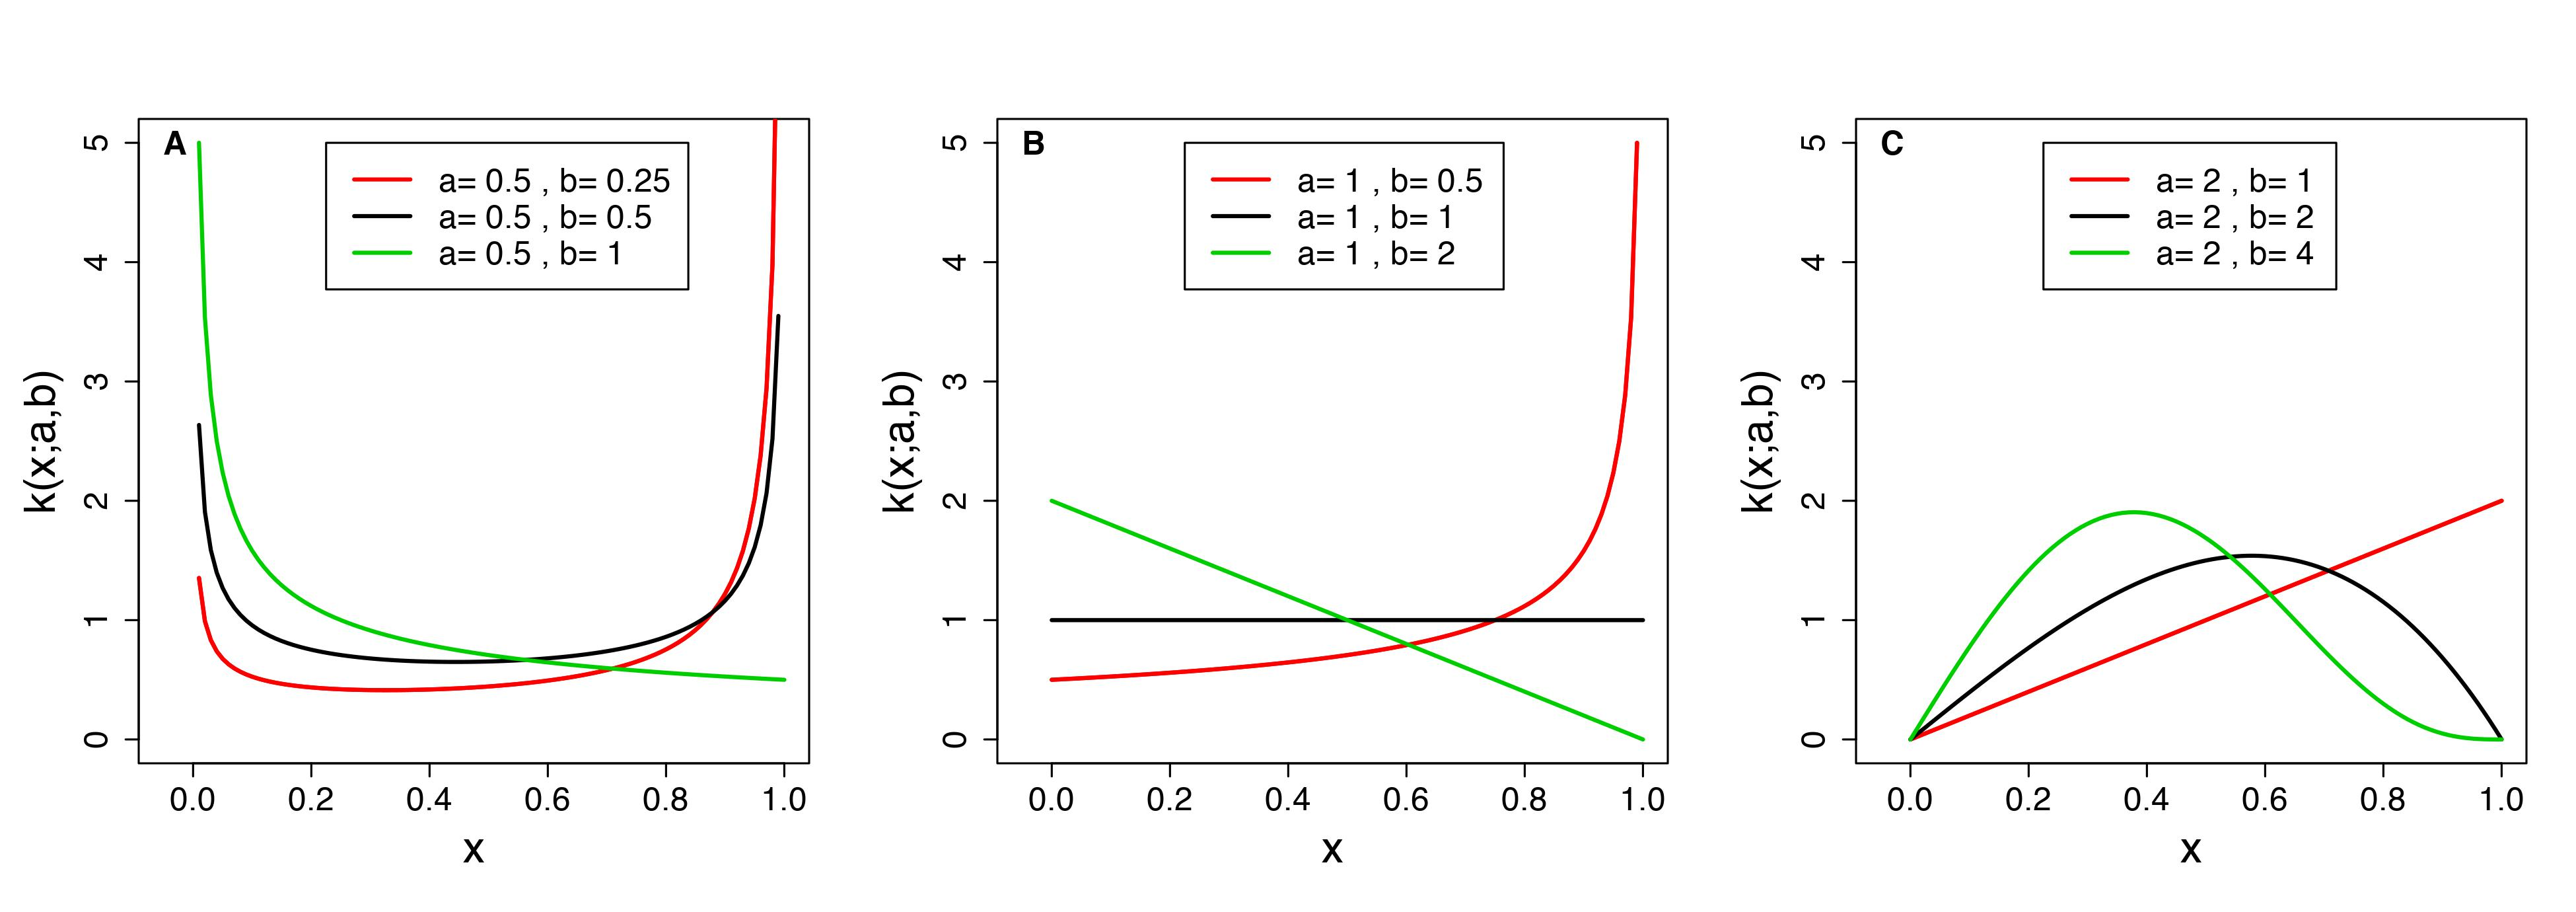
\includegraphics[scale=0.5,trim=0cm 0.25cm 0cm 0.25cm,clip]{pics/Epistasis/Kumar_dist.jpeg}
    \caption{Subset of Kumaraswamy distributions: each panel corresponds to a given value of $a$: $a<1$ in A produces distributions with an excess of extreme values as is often described about the distribution of fitness effects, $a=1$ in B represents simpler distributions, while $a=2$ in C encompasses bell-like distributions. The balance between low and high fitnesses is mainly determined by the ratio between $a$ and $b$: the higher $b$, the largest deleterious variants.}
    \label{fig:Kumar_dist}
\end{figure}

From the property connecting the Gamma function to factorial numbers for integer numbers -- $\Gamma(n+1)=n!$ -- it is straightforward to derive the steady-state fitness and its corollary mutational load when $a$ can be written under the form $1/k$ with $k \in \mathbb{N}^*$, which is given by:
\begin{align}
    \prec f^*_{\mathcal{K}_v(a,b)}\succ~=\prod _{i=1}^{1/a} \frac{2N_e/a+i}{2N_e/a+nb+i}
\end{align}

In parallel, it is also possible to determine an analytical solution when $a=2$ taking advantages of the well-known formula for half integers, which states that $\Gamma(m+1/2)=\frac{(2m)!}{2^{2m}m!}\sqrt{\pi}$ if $m \in \mathbb{N}^*$. Assuming that $nb$ is an integer, it is therefore possible to determine $\frac{\Gamma(N+1/2)}{\Gamma(N)}$ as well as $\frac{\Gamma(N+1/2+nb)}{\Gamma(N+nb)}$, which gives:
\begin{align}
    \prec f^*_{\mathcal{K}_v(2,b)}\succ~=2^{2nb}.\frac{(2N_e)!}{N_e!(N_e-1)!}.\frac{(N_e+nb)!(N_e+nb-1)!}{(2(N_e+nb))!}
    \label{eq_inter_fKura2}
\end{align}

Stirling's formula\footnote{As often happens in the History of Mathematics, Stirling's formula, despite its baptismal name, was not formulated first by Stirling but by De Moivre.} \citep{Dutka91} states that when $K$ is a large integer, the factorial matches the much simpler form $K!=\sqrt{2\pi K}(\frac{K}{e})^{n}$. Given that $\frac{(2K)!}{K!(K-1)!}=\frac{(2K)!K}{(K!)^2}$, substituting Stirling's formula in a term of the form found in Eq.(\ref{eq_inter_fKura2}) yields:
\begin{align*}
    \frac{(2K)!}{K!(K-1)!}\sim 2^{2K}\sqrt{\frac{K}{\pi}}\text{, for K} \in \mathbb{N}^*
\end{align*}

Finally, it yields for $a=2$ and $v=2(N_e-1)$:
\begin{align}
    \prec f^*_{\mathcal{K}_v(a,b)}\succ~=\sqrt{\frac{N_e}{N_e+nb}}
\end{align}

Using first order approximation, it follows from these findings that when $nb<<N_e$, the Poon-Otto's burden of complexity holds with $L^* ~\approx~ \frac{nb}{2N_e}$, which confirms that these confounding causes may be difficult to disentangle through data analysis alone. By contrast, if the number of interacting units is large, the mutational load can depart largely from this previous prediction, especially when $nb$ approaches or exceeds the order of magnitude of $N_e$. Noticeably, this new formulation shows that parameters $b$ (which can be seen as a mutational bias towards deleterious mutations) and $n$ are equally contributing to the load, and their importance critically depends on the shape of the neutral fitness distribution. Focusing on the most documented distributions, those displaying an excess of extreme values - both low and high ones potentially-, correspond to cases where the mutational load is increased if $b>1$, and decreased otherwise, for a given number of complementary units. But in contrast with Fisher's model, it seems plausible if not inevitable to assume that $n$ outnumbers small or even intermediate $N_e$ since each of the units can for instance represent an enzyme's or a protein's activity. 

\subsection{Discussion : how other biological features impact these predictions ?}

%To be put in the pesperctives part of the Obviously, there is a need to study higher and more realistic population sizes in order to draw robust conclusions.

Because the aim of this new framework is to try and understand the influence of epistasis from physical and chemical first principles, further developments will definitely need include other relevant features that should influence evolutionary outcomes. First, it is known that mutations occurring on coding sequences, even being synonymous, are rarely exactly neutral, reflecting in particular the cost arising from codon usage bias \citep{Ikemura85,Galtier18,laBella19}, a feature that definitely influences fitness landscapes \citep{Fragata18}. In parallel, not all kind of phenotypic traits undergo deleterious mutational biases as simple as that presented up until now : this is especially true for levels of expression\footnote{And organic shapes, albeit for different reasons.},  which often result themselves from complex changes in gene networks features such as the level of trans-regulatory elements, their affinity and specificity, and a pleitropic set of relations with cis-regulatory elements involving the whole genome \citep{Hodgkin98,Chesmore16,Boyle17,Sella19}. For illustrative purpose, let us imagine that a given gene is mainly regulated by a transcriptional inhibitor: as transcription factors face a mutational bias towards lower affinities, this bias should enhance gene expression rather than decrease it. Last but not least, if biological systems may be thought to be under directional selection to maximize growth and biomolecules production, the intertwining of pathways and biological reactions is more likely to result in a slightly different picture - portrayed on Figure \ref{fig:stab-mim} - than that displayed by a simple positive complementary epistasis: proteins that are too efficient may at some point yield collateral damages either because they monopolize resources in vain or as they induce toxicity (\textit{eg.} producing too many metabolites) \citep{Lilja17,Niehaus20,Labourel21}. Consequently, it seems more realistic that each of the non-worst genes is under more or less relaxed stabilizing selection towards an optimum, coinciding with the worst gene  -  that can only change when the worst gene of the set improves to a higher value - which means that even when no mutational bias exists, most genes involved in complementary epistasis should be pulled towards the worst one, for complementary epistasis becomes negative in those cases. Likewise, it seems judicious to study whether the effect of such epistasis differs when it occurs within entities part of a linear system or between parallel entities (which could of course be made by lower-level entities themselves) like two pathways comprised of proteins, which would also be philosophically interesting for its shared similarity with electric or heat systems - as recently outlined by \citet{Yi19} - where parallel and series circuit were shown to work differently a long while ago, by the then student Gustav Kirchhoff \citep{Charbonneau14}.\\

\begin{figure}[h!]
    \centering
    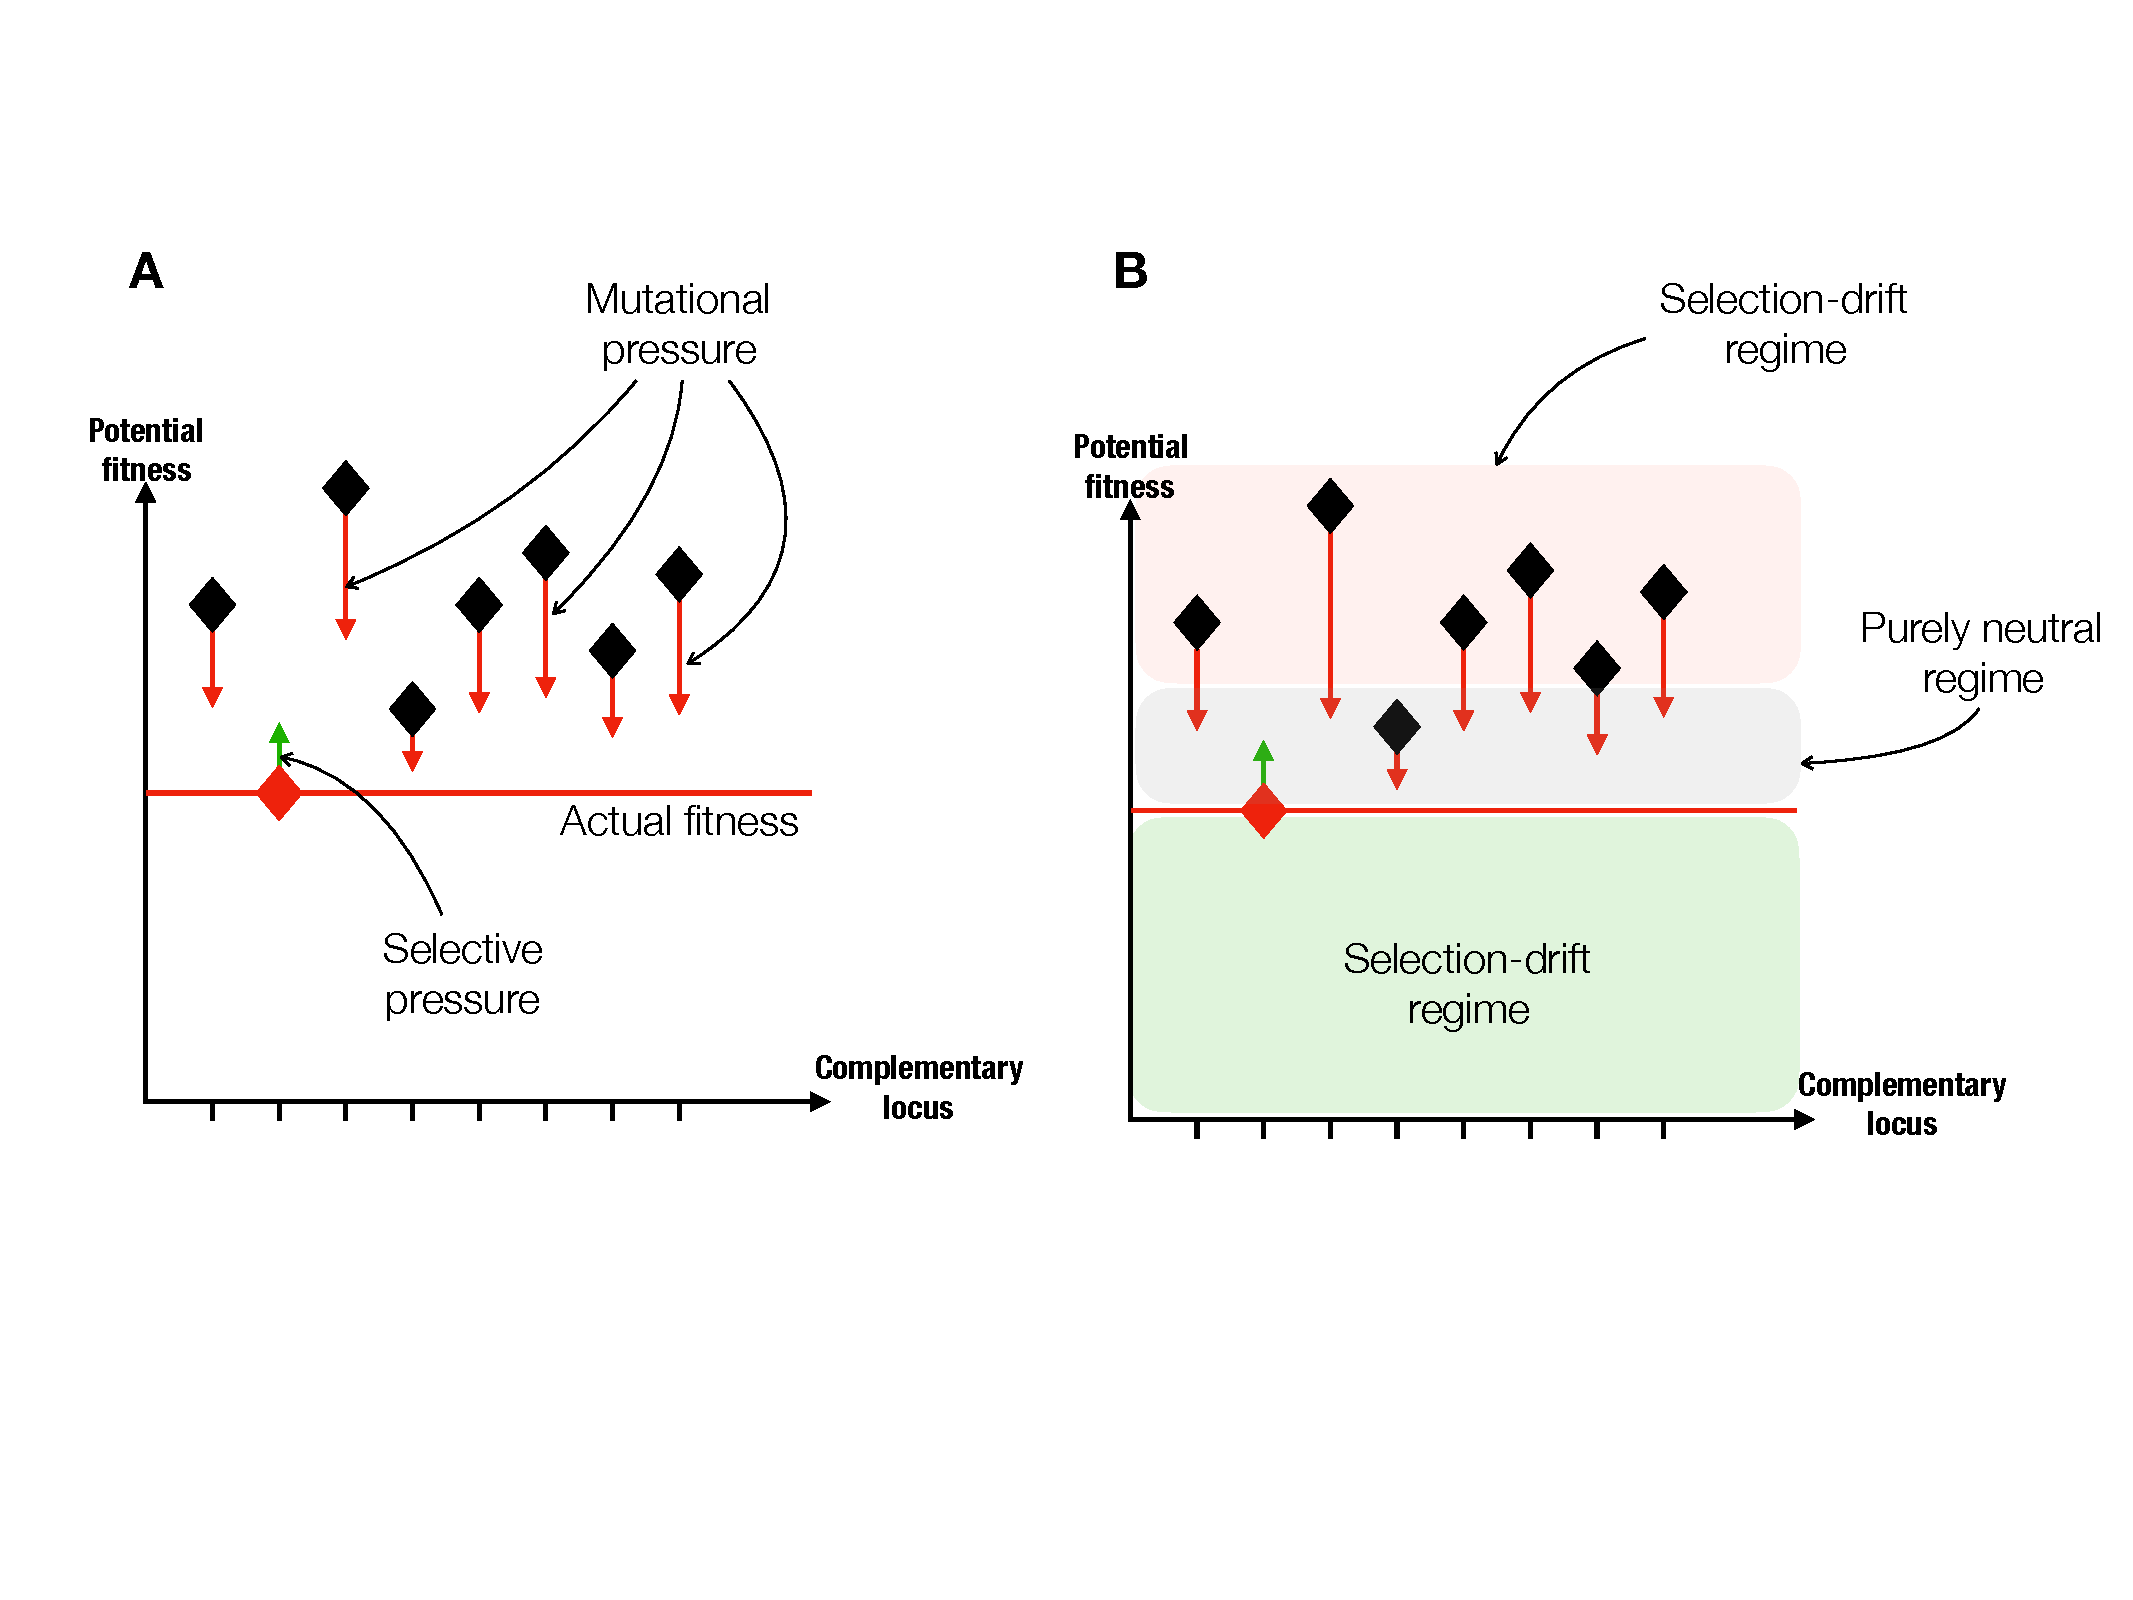
\includegraphics[scale=0.45,trim=1cm 7cm 0cm 4cm,clip]{pics/Epistasis/Stabilizing-mimetism.pdf}
    \caption{Owing to mutational biases, the mutational process exerts a pressure towards lower fitness phenotypes (A), which is not counterbalanced by Natural Selection above the actual fitness: this phenomenon may look like stabilizing selection since most mutations are going to stabilize the actual phenotype by pushing all loci towards the same lowest level coinciding with actual fitness. But in fact, it is even likely that mutations towards very high values of potential fitness can often prove to be deleterious rather than neutral (\textit{eg.} an enzyme far more efficient than its neighbours in a pathway may produce a metabolite so quickly that it ends up reaching toxic cellular levels.). In turn, only a small range of adaptive phenotypes exists at any given time (B). Despite the trait being under directional selection, this latter process thence mimics stabilizing selection, although towards an optimal area rather than a precise point, whilst the mutational pressure further stabilizes the actual deleterious phenotype.}
    \label{fig:stab-mim}
\end{figure}

Being directly based on functional insights, such a framework seems very relevant to start tackling the challenges set out by the joint evolution between basic functional epistasis -- and more broadly, genetic interactions -- and Adaptation from a population genetics theoretical perspective insofar as it may allow to draw very general and testable conclusions. In spite of its apparent specificity, it can indeed describe both intra-level and multilevel evolution: it is appropriate to describe the joint evolution of organs/appendages, as well as enzymes along a pathway, or organs/appendages and enzymes all together, provided that one knows how the genotype-phenoype-fitness map builds up. Many further developments are thereby possible.

One natural sequel would of course be to refine its components and account for the existence of compensatory mutations entailed by the multidimensional phenotypic redundancy of some biological features: higher enzyme concentrations can buffer lower kinetic enzymes - though it comes with the cost of a protein burden \citep{Koch83,Dill11,Kafri16}; villi can theoretically relax the selective pressure acting on enzymes for the absorption of nutrients; a longer calf can compensate for a smaller thigh or vice-versa, etc. To expand further in this area, it would also be relevant to see what happens when genes undergoing true stabilizing selection come into play, as they are also widespread\footnote{This is noticeably interesting for such fitness landscapes - including stabilizing selection - have been empirically documented in the case of drug resistance in microorganisms \citep{Ford20}.}\citep{Sella19}, and whether the joint evolution with the fitness effects of mutations - whose distribution both impacts the course and the outcome of Evolution while inescapably being subject to It - could overturn expectations.

However, it would seem premature to further investigate these specific building blocks more than others while we know that there exists plenty other kind of genetic interactions (\textit{eg.} biological modularity \citep{Wagner96}), that each deserves to be accounted for on a mechanistic basis: for instance, pleiotropy is, like epistasis and the distribution of fitness effects, both a result of Evolution and an intrinsic biological phenomenon \citep{Wagner96,Chesmore16} depending on its underpinnings, which are numerous. This means that understanding its joint evolution with epistasis requires first to inform which part is intrinsic to biological systems\footnote{In order to avoid introducing constraints which may be the result of Evolution, be it adaptive or not.}, when and how it can be alleviated, and how it finally impacts the genotype-phenotype-fitness map before these systems are studied using a complete framework, which undeniably sketches a rather more distant objective.%A first step of the project would therefore aim to deal analytically with simple instances of this model\footnote{Fisher's geometric model or Kaufman's NK complexity model seem well suited to feed into the thinking, but at this stage, it is not possible to state if they can properly translate the model assumptions.}, an approach which could then be further refine through simulations to study cases where analytic tools fail to yield predictions. This step should be the main subject of a first research article and comes with many perspectives.

Instead, it seems more appropriate to adopt a step-by-step approach where population genetics and first principle fitness landscapes are built in parallel, as was done in the past to understand the evolution of stability \citep{Taverna02,Bloom04} and its evolutionary \citep{Drummond05,Bloom06,Drummond08,Tokuriki09,Serohijos12,Dasmeh14,Echave17a} and functional consequences \citep{Bloom07,Geiler-Samerotte11,Dasmeh18}, and to derive the models of genetic interactions and constraints from these latter ones rather than taking them for granted because they currently exist after billion years of evolutionary history.% This would be the purpose of the second part of this project.

%\section{{Testing the framework and improving functional hypothesis through the evolution of enzymes embedded in pathways}\label{sec:TFEE}} PARTIE A RETRAVAILLER EN DISCUSSION DE LA PARTIE RESULTATS SUIVANTE

%Thereafter, the second step of the project could aim at studying how cellular fitness emerges as the intertwining of metabolic fluxes within a cell and how this relationship in turn influences enzyme evolution. Such a task would therefore intend to see how basic theoretical predictions match those explicitly modelling mechanisms, and contribute to draw conclusions about higher level constraints that population genetics approaches must take into account. It could build on insights from a previous approach that was recently built to prove that an enzyme's selective pressure is driven by several biochemical and ecological factors \citep{Labourel21}, which explain why their enzyme kinetic features resemble a zoo \citep{Bar-Even11,Davidi18} and seem far off physical optima if not sloppy \citep{Bar-Even15}. Noticeably, an enzyme's selective pressure partly relies on the efficiency of more upstream enzymes and the other way around, which fully legitimates to study theoretically the influence of complementary epistasis (as also do other models and experiments we already mentioned). Perhaps more importantly yet, because fitness relied on specific parts of pathways, our conclusions point to the need of looking deeper into how epistasis builds up in a pathway (series epistasis\footnote{\label{n1}In terms of electric/heat analogy.}) and between them (parallel epistasis\footnoteref{n1}), as well as it provides a framework to test ideas about the emergence and the further evolution of metabolic pathways.

%As stated in the introduction, some authors have already raised the need to address the consequences of high order epistasis - see \citep{Weinreich13} for instance - in the context of molecular evolution. In fact, \citet{Heckmann18} have lately tried to do so precisely in the case of enzyme kinetic parameters (focusing on turn-over numbers \(k_{cat}\)s). In their model relying on FBA\footnote{Flux Balance Analysis.}, the fitness of \textit{E.coli} cells results from the complex combination of thousands of enzymes whose \(k_{cat}\)s can undergo mutations. Mutation fixation of one variant is computed by a random draw from a binomial distribution with \citet{Kimura62}'s formula for fixation probability. Through that framework, they did observe that Evolution fails to produce optimal enzymes but this is mainly due to the premise that some enzymes are constrained under an efficiency ceiling, so that their study, though promising, does not provide a reliable answer to the influence of epistasis on Adaptation in the case of enzymes. This is even truer since FBA is already the fruit of a long evolutionary process and should therefore not be considered the appropriate framework to understand the joint evolution between epistasis and Adaptation.

%Previously, the Evolution of enzymes and pathways had usually been studied theoretically using the Flux Control Theory \citep{Kacser73,Heinrich74,Hartl85,Dean86}, where diminishing returns effects on flux are the result of complementary epistasis (named differently) because of the flux summation theorem \citep{Kacser73,Kacser95,Kaltenbach14}: this latter states that flux control has to be spread between all enzymes of a pathway. Though it is only valid under certain circumstances \citep{Bagheri-Chaichian03}, this theory has met some empirical success \citep{Dykhuizen90, Fell92} but came short of explaining why the system does not improve further its observed state since some enzymes - especially transporters among empirically documented cases \citep{Kacser81,Hartl85,Yi19} - necessarily have a large control and should therefore lead to a step-by-step increase through which large control coefficients continuously travel from one enzyme to another. Besides, the fact that transporters play a specific role is also puzzling and needs a careful examination for it can reflect many distinct causes (physical constraints limiting their efficiency through trade-offs \citep{Gudelj10,Bosdriesz18}, cellular constraints acting on metabolite and enzymatic content that, along with  organisms evolving under stabilizing selection for the efficiency of reactions, favour upstream control \citep{Wright10} are explanations that have been proposed in the past; but they are, in one way or another, \textit{ad hoc} assumptions).

%Surely, enzymes - and more generally proteins - face physical constraints at a point that prevents them from being more efficient, but this does not explain why the same enzyme can be more efficient -- both \textit{in vitro} and \textit{in vivo} \citep{Bar-Even11,Davidi16,Davidi18} -- in another species by many orders of magnitude and the fact that their kinetic activity can also be improved through readily evolvable levels of expression seems to contradict this argument and lends credence to initiatives trying to map fitness from first principles \citep{Bershtein17}. And even when these constraints are relevant, they have to be modelled in order to assess their influence. What we propose to do here is to build a model where fitness results from the flux sustained by different pathways and is initiated by nutrients for which cells are in competition alike it occurs in Nature. As a first approach relevant for theoretical purposes, a metabolic pathway can be modelled as a succession of more or less reversible Michaelis Menten reactions initiated by a transport process \citep{Labourel21}, according to the following scheme comprised of one initiating transport step followed by $n$ reversible reactions: 

%\small
%\begin{align}
 %\schemestart
 %\ch{$S_{j,env}$ + $T_j$}
  %\arrow{<=>[*0]}[0]
 %$S_j$ + $E_{j,1}$
 %\arrow{<=>[*0]}[0]
% $P_{j,1}$+$E_{j,2}$
 %\arrow{<=>}[0]
% (...)
 %\arrow(@c1--){->[*0$\eta_d$]}[-90]
% \arrow{<=>}[0]
% $P_{j,n-1}$+$E_{j,n}$
% \arrow{<=>}[0]
% P$_{j,f}$ ,
%\schemestop
%\label{chemMFluxGen}
%\end{align}
%\normalsize

%with $j$ denoting the $j^{ieth}$ nutrient, $S_{j,env}$ and $S_j$ corresponding to the environmental and the cellular substrate ($j$), $T_j$ and $E_{j,i}$ representing respectively the transporter protein and the $i_{eth}$ enzyme of the pathway involved in processing substrate $S_j$, while $P_{j,f}$ represents the final product of this pathway (\textit{eg.} energy).

%The first step of the model would intend to determine the evolutionary outcomes at mutation-selection-drift balance, how fitness builds up from the different enzymes and whether there is space for evolutionary contingency or not. To do so, one should model the joint evolution of enzymes embedded in one such pathway, where fitness is represented by the final point: the efficiency of enzymes derives from its kinetic parameters and its concentration, while the need for an efficient enzyme (\textit{i.e.} the fitness landscape on which it evolves) is driven by the extra flux it provides. It needs to account for possible loss of fitness due to excessive concentrations of metabolite (for instance, because it creates an imbalance with ubiquitous promiscuous reactions\citep{Khersonsky10,Peracchi18,Tawfik20,Niehaus20}), and that contingent to the protein burden related to the cost of expression, and, to a lesser point, cellular and membrane molecular crowding \citep{Chou14,Labourel21}. It also needs to include noise in gene expression as noisiness was shown to harbour a potential for very deleterious effects on such systems\citep{Wang11} - not to mention that some concentrations are biochemically unachievable - that should be contingent to cell sizes \citep{Labourel21} in such a way that evolutionary outcomes must be sensitive to this latter parameter.

%The follow-up step of this project would be to unveil what occurs when there are multiple pathways that contribute to a cell's fitness under diverse circumstances (pathways could be parallel or branched, fitness could be determined only by the last step of processes, like for phospholipid synthesis, or result from multiple additions that add along the pathway, like for energy). With these latter realistic components, there would emerge a need to synchronize pathways in order for cells to be efficient and ensure them, in particular, to avoid some adverse effects of over-competitiveness: the intrinsic constraint of epistasis would therefore concern two different levels of interactions. Interestingly, if we also explicitly introduce substrate competition, we may see that some cells sacrifice part of their functions in order to maximize their fitness. This should be especially true when the environment is considered dynamically and can be depleted by cells, because cells may rather feed on nutrients than produce them \textit{de novo}: determining when it happens and which cellular constraints (membrane crowding, protein burden) drive the process would open up avenues about the evolutionary trajectories that followed from the advent of the eukaryotic cell or transitions towards multicellularity.\\

%Concurrently, it has been established that the ability of a protein to fold and adopt its active conformation is a prerequisite to an enzyme's function \citep{Taverna02,Bloom04,Echave17a}, not to mention that misfolded states conceals the potential to be harmful \citep{Bucciantini02,Geiler-Samerotte11}. Accounting for the fact that enzymes cannot sacrifice too much stability \citep{Taverna02} subsequently enabled the community to better understand many processes in molecular evolution, such as the distribution of evolutionary rates or the effects of mutations \citep{Zeldovich07,Tokuriki07,Lobkovsky10,Tokuriki09,Echave17a,Bershtein17}, and led to insights about the evolvability of new functions \citep{Bloom04,Bloom06,Tokuriki08}. Meanwhile, it has been documented that mutations are on average destabilizing \citep{Tokuriki07,Tokuriki08} so that it gives rise to an apparent function-stability trade-off \citep{Shoichet95,DePristo05,Weinreich06,Lunzer10}, which can preclude many enzymes to be highly efficient \citep{Tomala19}. It has thus become increasingly apparent that understanding enzyme (and pathway) evolution crucially requires to integrate both these fitness components. At this stage however and in spite of commendable first proposals \citep{Bloom04}, combining mechanistically the effects of residues on stability and catalysis - through their contribution to the respective $\Delta G$ - within a general framework remains a major challenge \citep{Echave17a,Bershtein17} because the intensity of the trade-off and its existence itself\footnote{As many residues act specifically on stability, they can even buffer some of the deleterious effects of mutations affecting both \citep{Tokuriki09,Storz18}.} seem to be largely enzyme-dependent \citep{Schreiber94,Burg02,Knies17,Miller17,Tomala19}, and it is also anything but obvious to draw a two-dimensional phenotype-fitness map involving both these quantities (see \citep{Echave19} for one of the most recent and significant efforts relying on the ansatz of neutral threshold in the fitness landscapes). Thence, this issue of bringing together stability and catalysis still calls for more in-depth reflection to pick the right way to capture its founding principles, and, in turn, the arising evolutionary consequences for the question at hand.

%Because there are many dimensions that contribute to enzymes, the project may have to be split into two different research articles, the first one focusing on the effect of epistasis and competition, while the second would seek to bring together enzyme activity and stability within a single evolutionary framework. Such a model could be used later to test ideas not only about the evolution of the lower level entities embodied by proteins but also for the upper level entities constituted by pathways, as well as this could be a starting point to tackle the influence of the same mechanism when it concerns cells, another kind of essentially fungible entities \citep{Grosberg07}. It should also be useful to understand some patterns in molecular evolution because it has been shown that rates of Evolution are determined by a complex functional-stability relationship \citep{Marcos15,Echave16,Jack16,Jimenez18}, and also that highly expressed enzymes evolve more slowly \citep{Drummond05,Drummond08,Serohijos12}. Understanding what in the first place governs an enzyme's level of expression would therefore be useful to predict evolutionary rates - at least in the case of enzymes - and, coupled with the activity-stability gradient \citep{Echave19}, it may shed light on questions that are contingent to these estimates.
\newpage
\subsubsection*{Appendix - simulation outcomes for $N_e=10$}

\begin{figure}[h!]
    \centering
    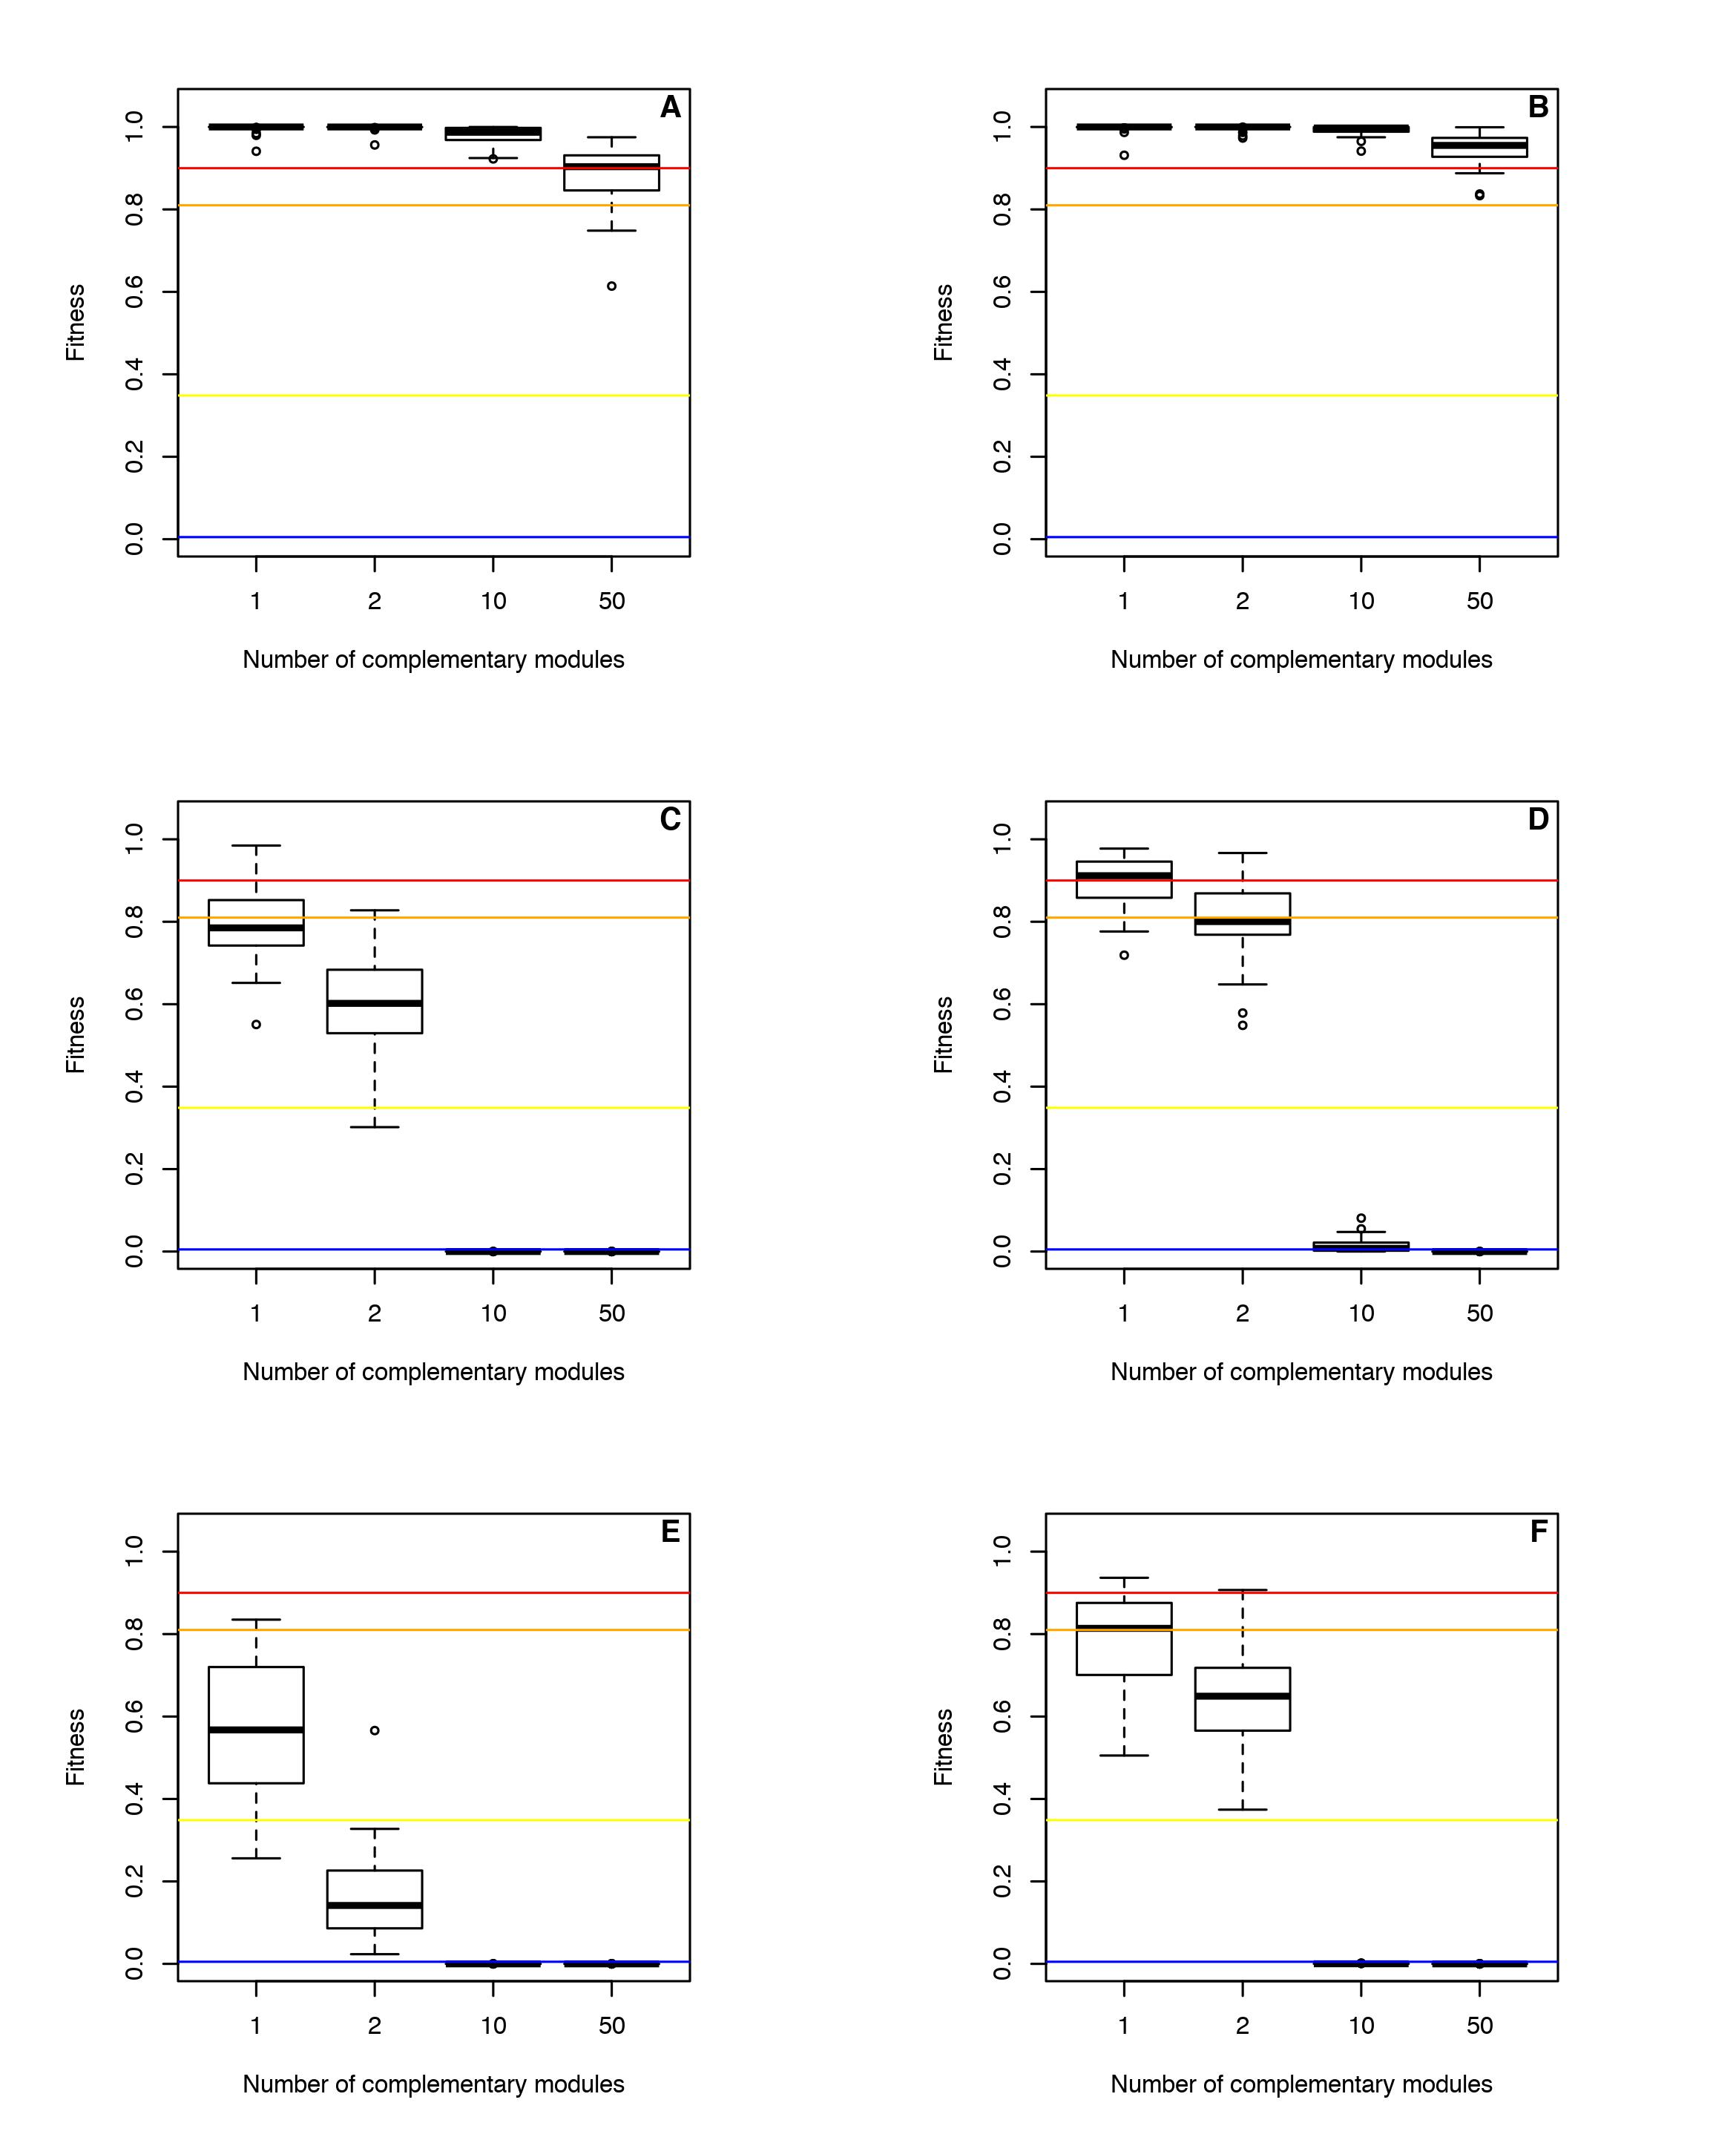
\includegraphics[scale=0.75,trim=0cm 0cm 0cm 0cm,clip]{pics/Epistasis/Evo_Outcomes_Ne10.jpeg}
    \caption{Simulation outcomes for the mutation-election-drift balance with $N_e=10$ when the interplay of complementary epistasis and diminishing returns epistasis (through the fitness landscape of traits) are accounted for. The number of complementary modules varies from 1 to 50. Each line corresponds to a level of mutational bias: null in (A) and (B), low in (C) and (D), high in (E) and (F) - see text for details; each column represents a level of mutational variability, with (A), (C) and (E) having low variability while (B), (D) and (F) display a moderate to high variability.}
    \label{fig:Outcomes10}
\end{figure}

%\end{document}
